\documentclass[twoside]{book}

% Packages required by doxygen
\usepackage{calc}
\usepackage{doxygen}
\usepackage{graphicx}
\usepackage[utf8]{inputenc}
\usepackage{makeidx}
\usepackage{multicol}
\usepackage{multirow}
\usepackage{textcomp}
\usepackage[table]{xcolor}

% Font selection
\usepackage[T1]{fontenc}
\usepackage{mathptmx}
\usepackage[scaled=.90]{helvet}
\usepackage{courier}
\usepackage{amssymb}
\usepackage{sectsty}
\renewcommand{\familydefault}{\sfdefault}
\allsectionsfont{%
  \fontseries{bc}\selectfont%
  \color{darkgray}%
}
\renewcommand{\DoxyLabelFont}{%
  \fontseries{bc}\selectfont%
  \color{darkgray}%
}

% Page & text layout
\usepackage{geometry}
\geometry{%
  a4paper,%
  top=2.5cm,%
  bottom=2.5cm,%
  left=2.5cm,%
  right=2.5cm%
}
\tolerance=750
\hfuzz=15pt
\hbadness=750
\setlength{\emergencystretch}{15pt}
\setlength{\parindent}{0cm}
\setlength{\parskip}{0.2cm}
\makeatletter
\renewcommand{\paragraph}{%
  \@startsection{paragraph}{4}{0ex}{-1.0ex}{1.0ex}{%
    \normalfont\normalsize\bfseries\SS@parafont%
  }%
}
\renewcommand{\subparagraph}{%
  \@startsection{subparagraph}{5}{0ex}{-1.0ex}{1.0ex}{%
    \normalfont\normalsize\bfseries\SS@subparafont%
  }%
}
\makeatother

% Headers & footers
\usepackage{fancyhdr}
\pagestyle{fancyplain}
\fancyhead[LE]{\fancyplain{}{\bfseries\thepage}}
\fancyhead[CE]{\fancyplain{}{}}
\fancyhead[RE]{\fancyplain{}{\bfseries\leftmark}}
\fancyhead[LO]{\fancyplain{}{\bfseries\rightmark}}
\fancyhead[CO]{\fancyplain{}{}}
\fancyhead[RO]{\fancyplain{}{\bfseries\thepage}}
\fancyfoot[LE]{\fancyplain{}{}}
\fancyfoot[CE]{\fancyplain{}{}}
\fancyfoot[RE]{\fancyplain{}{\bfseries\scriptsize Generated on Thu Aug 20 2015 09\-:26\-:34 for End User Flash Tool by Doxygen }}
\fancyfoot[LO]{\fancyplain{}{\bfseries\scriptsize Generated on Thu Aug 20 2015 09\-:26\-:34 for End User Flash Tool by Doxygen }}
\fancyfoot[CO]{\fancyplain{}{}}
\fancyfoot[RO]{\fancyplain{}{}}
\renewcommand{\footrulewidth}{0.4pt}
\renewcommand{\chaptermark}[1]{%
  \markboth{#1}{}%
}
\renewcommand{\sectionmark}[1]{%
  \markright{\thesection\ #1}%
}

% Indices & bibliography
\usepackage{natbib}
\usepackage[titles]{tocloft}
\setcounter{tocdepth}{3}
\setcounter{secnumdepth}{5}
\makeindex

% Hyperlinks (required, but should be loaded last)
\usepackage{ifpdf}
\ifpdf
  \usepackage[pdftex,pagebackref=true]{hyperref}
\else
  \usepackage[ps2pdf,pagebackref=true]{hyperref}
\fi
\hypersetup{%
  colorlinks=true,%
  linkcolor=blue,%
  citecolor=blue,%
  unicode%
}

% Custom commands
\newcommand{\clearemptydoublepage}{%
  \newpage{\pagestyle{empty}\cleardoublepage}%
}


%===== C O N T E N T S =====

\begin{document}

% Titlepage & ToC
\hypersetup{pageanchor=false}
\pagenumbering{roman}
\begin{titlepage}
\vspace*{7cm}
\begin{center}%
{\Large End User Flash Tool }\\
\vspace*{1cm}
{\large Generated by Doxygen 1.8.6}\\
\vspace*{0.5cm}
{\small Thu Aug 20 2015 09:26:34}\\
\end{center}
\end{titlepage}
\clearemptydoublepage
\tableofcontents
\clearemptydoublepage
\pagenumbering{arabic}
\hypersetup{pageanchor=true}

%--- Begin generated contents ---
\chapter{Hierarchical Index}
\section{Class Hierarchy}
This inheritance list is sorted roughly, but not completely, alphabetically\-:\begin{DoxyCompactList}
\item \contentsline{section}{Data\-Gatherer}{\pageref{classDataGatherer}}{}
\item \contentsline{section}{Flasher}{\pageref{classFlasher}}{}
\item Q\-Dialog\begin{DoxyCompactList}
\item \contentsline{section}{About}{\pageref{classAbout}}{}
\item \contentsline{section}{Add\-Component}{\pageref{classAddComponent}}{}
\item \contentsline{section}{Choose\-Chip}{\pageref{classChooseChip}}{}
\item \contentsline{section}{Delete\-Components}{\pageref{classDeleteComponents}}{}
\item \contentsline{section}{Info\-Dialog}{\pageref{classInfoDialog}}{}
\item \contentsline{section}{Preferences}{\pageref{classPreferences}}{}
\item \contentsline{section}{Supported}{\pageref{classSupported}}{}
\end{DoxyCompactList}
\item Q\-Main\-Window\begin{DoxyCompactList}
\item \contentsline{section}{Main\-Window}{\pageref{classMainWindow}}{}
\end{DoxyCompactList}
\item Q\-Object\begin{DoxyCompactList}
\item \contentsline{section}{Test\-\_\-1}{\pageref{classTest__1}}{}
\end{DoxyCompactList}
\item Q\-Sort\-Filter\-Proxy\-Model\begin{DoxyCompactList}
\item \contentsline{section}{Multi\-Sort\-Filter\-Model}{\pageref{classMultiSortFilterModel}}{}
\end{DoxyCompactList}
\item \contentsline{section}{qt\-\_\-meta\-\_\-stringdata\-\_\-\-About\-\_\-t}{\pageref{structqt__meta__stringdata__About__t}}{}
\item \contentsline{section}{qt\-\_\-meta\-\_\-stringdata\-\_\-\-Add\-Component\-\_\-t}{\pageref{structqt__meta__stringdata__AddComponent__t}}{}
\item \contentsline{section}{qt\-\_\-meta\-\_\-stringdata\-\_\-\-Choose\-Chip\-\_\-t}{\pageref{structqt__meta__stringdata__ChooseChip__t}}{}
\item \contentsline{section}{qt\-\_\-meta\-\_\-stringdata\-\_\-\-Delete\-Components\-\_\-t}{\pageref{structqt__meta__stringdata__DeleteComponents__t}}{}
\item \contentsline{section}{qt\-\_\-meta\-\_\-stringdata\-\_\-\-Info\-Dialog\-\_\-t}{\pageref{structqt__meta__stringdata__InfoDialog__t}}{}
\item \contentsline{section}{qt\-\_\-meta\-\_\-stringdata\-\_\-\-Main\-Window\-\_\-t}{\pageref{structqt__meta__stringdata__MainWindow__t}}{}
\item \contentsline{section}{qt\-\_\-meta\-\_\-stringdata\-\_\-\-Multi\-Sort\-Filter\-Model\-\_\-t}{\pageref{structqt__meta__stringdata__MultiSortFilterModel__t}}{}
\item \contentsline{section}{qt\-\_\-meta\-\_\-stringdata\-\_\-\-Preferences\-\_\-t}{\pageref{structqt__meta__stringdata__Preferences__t}}{}
\item \contentsline{section}{qt\-\_\-meta\-\_\-stringdata\-\_\-\-Supported\-\_\-t}{\pageref{structqt__meta__stringdata__Supported__t}}{}
\item \contentsline{section}{qt\-\_\-meta\-\_\-stringdata\-\_\-\-Test\-\_\-1\-\_\-t}{\pageref{structqt__meta__stringdata__Test__1__t}}{}
\item \contentsline{section}{Ui\-\_\-\-About}{\pageref{classUi__About}}{}
\begin{DoxyCompactList}
\item \contentsline{section}{Ui\-:\-:About}{\pageref{classUi_1_1About}}{}
\end{DoxyCompactList}
\item \contentsline{section}{Ui\-\_\-\-Add\-Component}{\pageref{classUi__AddComponent}}{}
\begin{DoxyCompactList}
\item \contentsline{section}{Ui\-:\-:Add\-Component}{\pageref{classUi_1_1AddComponent}}{}
\end{DoxyCompactList}
\item \contentsline{section}{Ui\-\_\-\-Choose\-Chip}{\pageref{classUi__ChooseChip}}{}
\begin{DoxyCompactList}
\item \contentsline{section}{Ui\-:\-:Choose\-Chip}{\pageref{classUi_1_1ChooseChip}}{}
\end{DoxyCompactList}
\item \contentsline{section}{Ui\-\_\-\-Delete\-Components}{\pageref{classUi__DeleteComponents}}{}
\begin{DoxyCompactList}
\item \contentsline{section}{Ui\-:\-:Delete\-Components}{\pageref{classUi_1_1DeleteComponents}}{}
\end{DoxyCompactList}
\item \contentsline{section}{Ui\-\_\-\-Info\-Dialog}{\pageref{classUi__InfoDialog}}{}
\begin{DoxyCompactList}
\item \contentsline{section}{Ui\-:\-:Info\-Dialog}{\pageref{classUi_1_1InfoDialog}}{}
\end{DoxyCompactList}
\item \contentsline{section}{Ui\-\_\-\-Main\-Window}{\pageref{classUi__MainWindow}}{}
\begin{DoxyCompactList}
\item \contentsline{section}{Ui\-:\-:Main\-Window}{\pageref{classUi_1_1MainWindow}}{}
\end{DoxyCompactList}
\item \contentsline{section}{Ui\-\_\-\-Preferences}{\pageref{classUi__Preferences}}{}
\begin{DoxyCompactList}
\item \contentsline{section}{Ui\-:\-:Preferences}{\pageref{classUi_1_1Preferences}}{}
\end{DoxyCompactList}
\item \contentsline{section}{Ui\-\_\-\-Supported}{\pageref{classUi__Supported}}{}
\begin{DoxyCompactList}
\item \contentsline{section}{Ui\-:\-:Supported}{\pageref{classUi_1_1Supported}}{}
\end{DoxyCompactList}
\end{DoxyCompactList}

\chapter{Class Index}
\section{Class List}
Here are the classes, structs, unions and interfaces with brief descriptions\-:\begin{DoxyCompactList}
\item\contentsline{section}{\hyperlink{classAbout}{About} }{\pageref{classAbout}}{}
\item\contentsline{section}{\hyperlink{classUi_1_1About}{Ui\-::\-About} }{\pageref{classUi_1_1About}}{}
\item\contentsline{section}{\hyperlink{classAddComponent}{Add\-Component} }{\pageref{classAddComponent}}{}
\item\contentsline{section}{\hyperlink{classUi_1_1AddComponent}{Ui\-::\-Add\-Component} }{\pageref{classUi_1_1AddComponent}}{}
\item\contentsline{section}{\hyperlink{classChooseChip}{Choose\-Chip} }{\pageref{classChooseChip}}{}
\item\contentsline{section}{\hyperlink{classUi_1_1ChooseChip}{Ui\-::\-Choose\-Chip} }{\pageref{classUi_1_1ChooseChip}}{}
\item\contentsline{section}{\hyperlink{classDataGatherer}{Data\-Gatherer} }{\pageref{classDataGatherer}}{}
\item\contentsline{section}{\hyperlink{classDeleteComponents}{Delete\-Components} }{\pageref{classDeleteComponents}}{}
\item\contentsline{section}{\hyperlink{classUi_1_1DeleteComponents}{Ui\-::\-Delete\-Components} }{\pageref{classUi_1_1DeleteComponents}}{}
\item\contentsline{section}{\hyperlink{classFlasher}{Flasher} }{\pageref{classFlasher}}{}
\item\contentsline{section}{\hyperlink{classInfoDialog}{Info\-Dialog} }{\pageref{classInfoDialog}}{}
\item\contentsline{section}{\hyperlink{classUi_1_1InfoDialog}{Ui\-::\-Info\-Dialog} }{\pageref{classUi_1_1InfoDialog}}{}
\item\contentsline{section}{\hyperlink{classMainWindow}{Main\-Window} }{\pageref{classMainWindow}}{}
\item\contentsline{section}{\hyperlink{classUi_1_1MainWindow}{Ui\-::\-Main\-Window} }{\pageref{classUi_1_1MainWindow}}{}
\item\contentsline{section}{\hyperlink{classMultiSortFilterModel}{Multi\-Sort\-Filter\-Model} }{\pageref{classMultiSortFilterModel}}{}
\item\contentsline{section}{\hyperlink{classUi_1_1Preferences}{Ui\-::\-Preferences} }{\pageref{classUi_1_1Preferences}}{}
\item\contentsline{section}{\hyperlink{classPreferences}{Preferences} }{\pageref{classPreferences}}{}
\item\contentsline{section}{\hyperlink{structqt__meta__stringdata__About__t}{qt\-\_\-meta\-\_\-stringdata\-\_\-\-About\-\_\-t} }{\pageref{structqt__meta__stringdata__About__t}}{}
\item\contentsline{section}{\hyperlink{structqt__meta__stringdata__AddComponent__t}{qt\-\_\-meta\-\_\-stringdata\-\_\-\-Add\-Component\-\_\-t} }{\pageref{structqt__meta__stringdata__AddComponent__t}}{}
\item\contentsline{section}{\hyperlink{structqt__meta__stringdata__ChooseChip__t}{qt\-\_\-meta\-\_\-stringdata\-\_\-\-Choose\-Chip\-\_\-t} }{\pageref{structqt__meta__stringdata__ChooseChip__t}}{}
\item\contentsline{section}{\hyperlink{structqt__meta__stringdata__DeleteComponents__t}{qt\-\_\-meta\-\_\-stringdata\-\_\-\-Delete\-Components\-\_\-t} }{\pageref{structqt__meta__stringdata__DeleteComponents__t}}{}
\item\contentsline{section}{\hyperlink{structqt__meta__stringdata__InfoDialog__t}{qt\-\_\-meta\-\_\-stringdata\-\_\-\-Info\-Dialog\-\_\-t} }{\pageref{structqt__meta__stringdata__InfoDialog__t}}{}
\item\contentsline{section}{\hyperlink{structqt__meta__stringdata__MainWindow__t}{qt\-\_\-meta\-\_\-stringdata\-\_\-\-Main\-Window\-\_\-t} }{\pageref{structqt__meta__stringdata__MainWindow__t}}{}
\item\contentsline{section}{\hyperlink{structqt__meta__stringdata__MultiSortFilterModel__t}{qt\-\_\-meta\-\_\-stringdata\-\_\-\-Multi\-Sort\-Filter\-Model\-\_\-t} }{\pageref{structqt__meta__stringdata__MultiSortFilterModel__t}}{}
\item\contentsline{section}{\hyperlink{structqt__meta__stringdata__Preferences__t}{qt\-\_\-meta\-\_\-stringdata\-\_\-\-Preferences\-\_\-t} }{\pageref{structqt__meta__stringdata__Preferences__t}}{}
\item\contentsline{section}{\hyperlink{structqt__meta__stringdata__Supported__t}{qt\-\_\-meta\-\_\-stringdata\-\_\-\-Supported\-\_\-t} }{\pageref{structqt__meta__stringdata__Supported__t}}{}
\item\contentsline{section}{\hyperlink{structqt__meta__stringdata__Test__1__t}{qt\-\_\-meta\-\_\-stringdata\-\_\-\-Test\-\_\-1\-\_\-t} }{\pageref{structqt__meta__stringdata__Test__1__t}}{}
\item\contentsline{section}{\hyperlink{classUi_1_1Supported}{Ui\-::\-Supported} }{\pageref{classUi_1_1Supported}}{}
\item\contentsline{section}{\hyperlink{classSupported}{Supported} }{\pageref{classSupported}}{}
\item\contentsline{section}{\hyperlink{classTest__1}{Test\-\_\-1} }{\pageref{classTest__1}}{}
\item\contentsline{section}{\hyperlink{classUi__About}{Ui\-\_\-\-About} }{\pageref{classUi__About}}{}
\item\contentsline{section}{\hyperlink{classUi__AddComponent}{Ui\-\_\-\-Add\-Component} }{\pageref{classUi__AddComponent}}{}
\item\contentsline{section}{\hyperlink{classUi__ChooseChip}{Ui\-\_\-\-Choose\-Chip} }{\pageref{classUi__ChooseChip}}{}
\item\contentsline{section}{\hyperlink{classUi__DeleteComponents}{Ui\-\_\-\-Delete\-Components} }{\pageref{classUi__DeleteComponents}}{}
\item\contentsline{section}{\hyperlink{classUi__InfoDialog}{Ui\-\_\-\-Info\-Dialog} }{\pageref{classUi__InfoDialog}}{}
\item\contentsline{section}{\hyperlink{classUi__MainWindow}{Ui\-\_\-\-Main\-Window} }{\pageref{classUi__MainWindow}}{}
\item\contentsline{section}{\hyperlink{classUi__Preferences}{Ui\-\_\-\-Preferences} }{\pageref{classUi__Preferences}}{}
\item\contentsline{section}{\hyperlink{classUi__Supported}{Ui\-\_\-\-Supported} }{\pageref{classUi__Supported}}{}
\end{DoxyCompactList}

\chapter{Class Documentation}
\hypertarget{classAbout}{\section{About Class Reference}
\label{classAbout}\index{About@{About}}
}
Inheritance diagram for About\-:\begin{figure}[H]
\begin{center}
\leavevmode
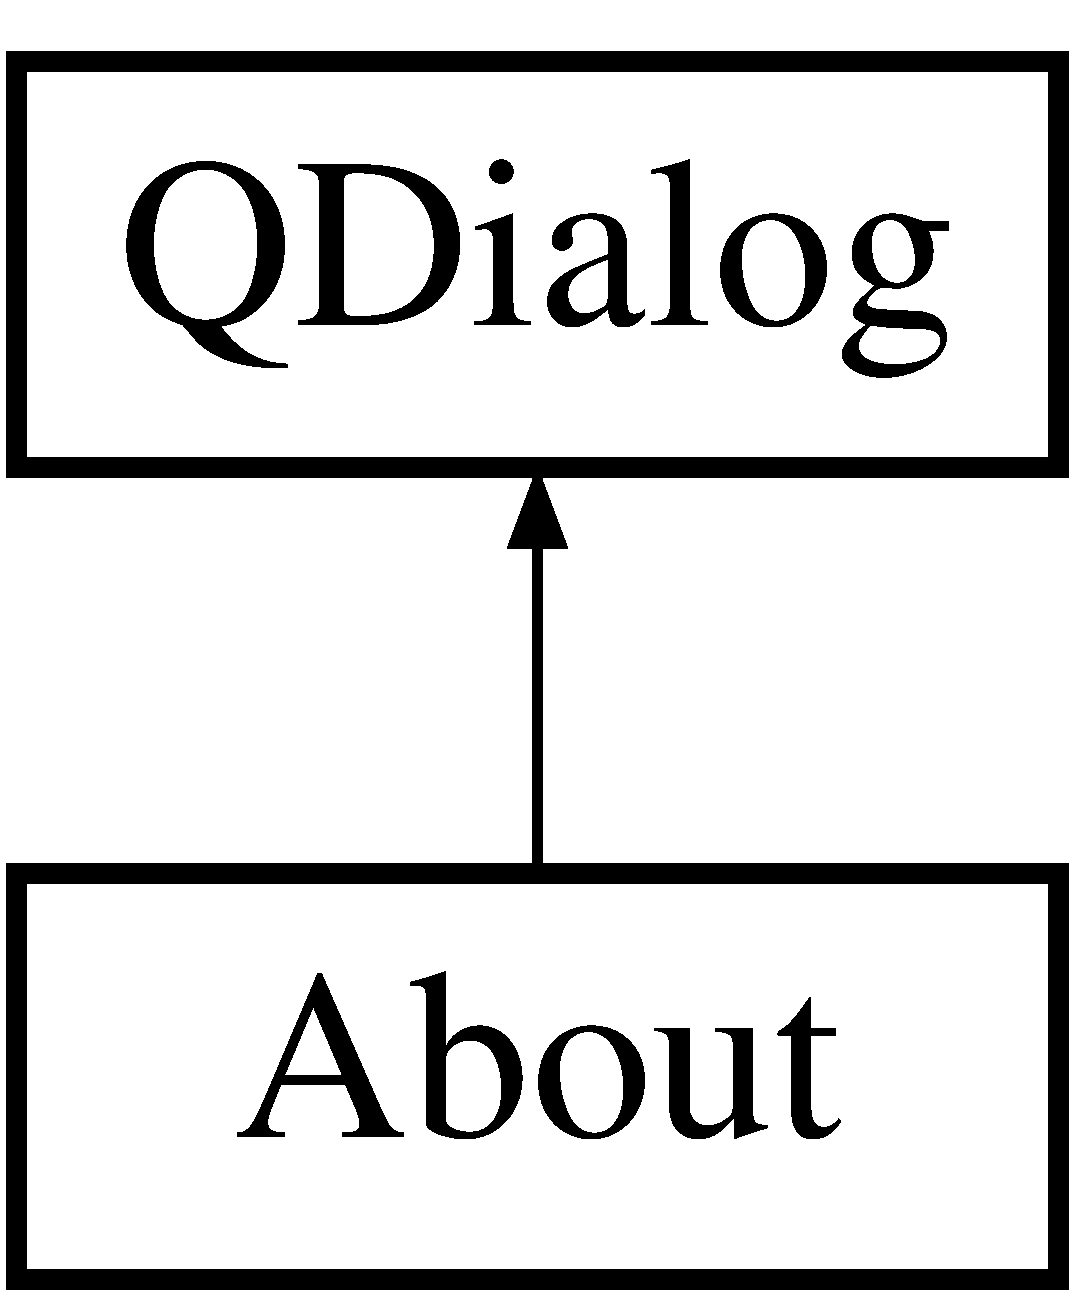
\includegraphics[height=2.000000cm]{classAbout}
\end{center}
\end{figure}
\subsection*{Public Member Functions}
\begin{DoxyCompactItemize}
\item 
\hypertarget{classAbout_ab79599ebbcdeffe0a96e00f010e64177}{{\bfseries About} (Q\-Widget $\ast$parent=0)}\label{classAbout_ab79599ebbcdeffe0a96e00f010e64177}

\end{DoxyCompactItemize}


The documentation for this class was generated from the following files\-:\begin{DoxyCompactItemize}
\item 
about.\-h\item 
about.\-cpp\end{DoxyCompactItemize}

\hypertarget{classUi_1_1About}{\section{Ui\-:\-:About Class Reference}
\label{classUi_1_1About}\index{Ui\-::\-About@{Ui\-::\-About}}
}
Inheritance diagram for Ui\-:\-:About\-:\begin{figure}[H]
\begin{center}
\leavevmode
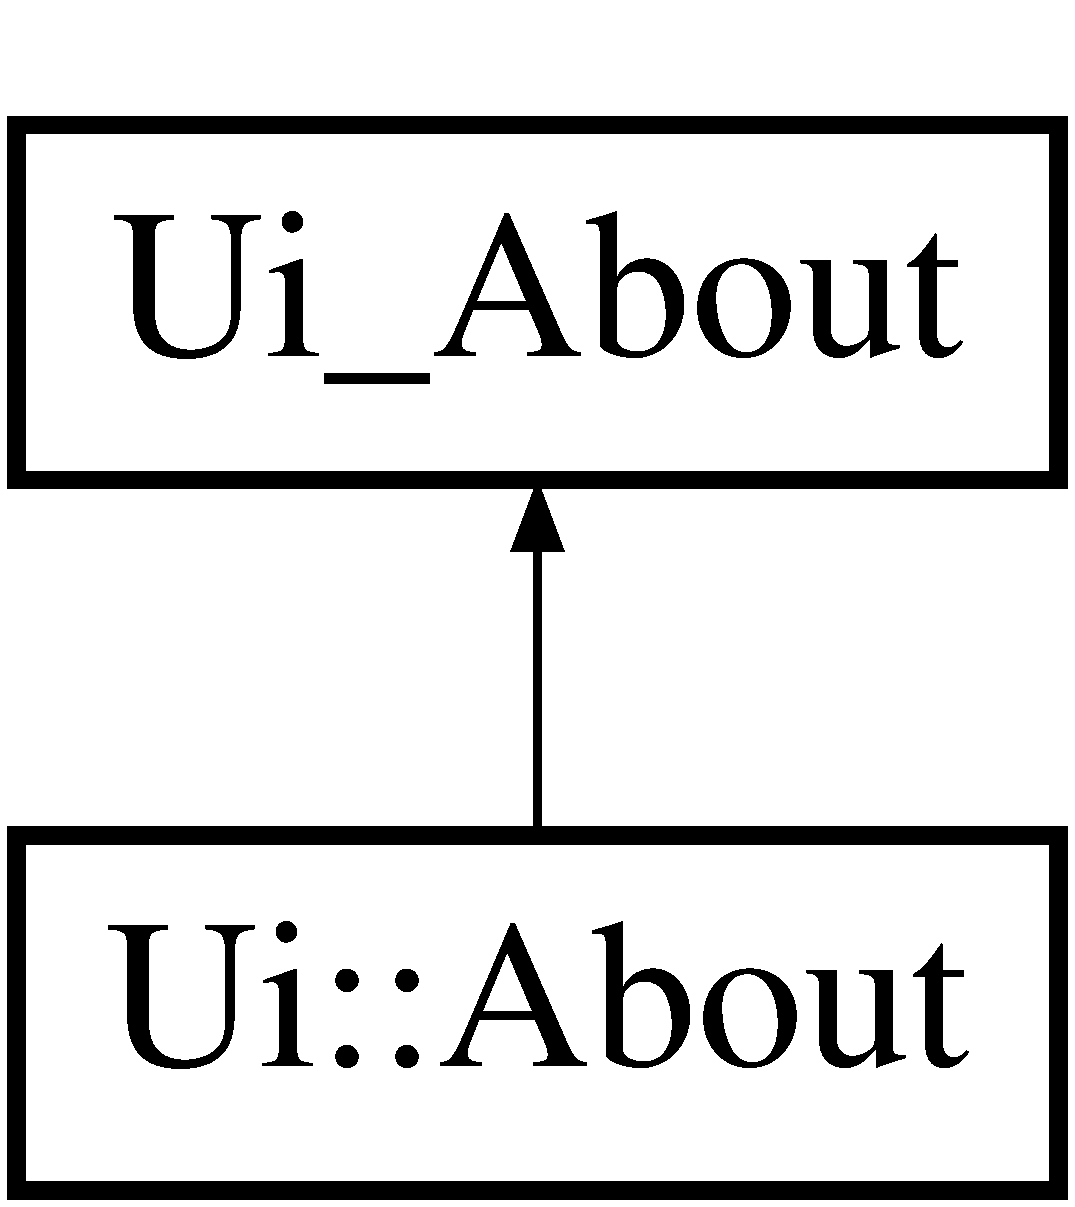
\includegraphics[height=2.000000cm]{classUi_1_1About}
\end{center}
\end{figure}
\subsection*{Additional Inherited Members}


The documentation for this class was generated from the following file\-:\begin{DoxyCompactItemize}
\item 
ui\-\_\-about.\-h\end{DoxyCompactItemize}

\hypertarget{classAddComponent}{\section{Add\-Component Class Reference}
\label{classAddComponent}\index{Add\-Component@{Add\-Component}}
}
Inheritance diagram for Add\-Component\-:\begin{figure}[H]
\begin{center}
\leavevmode
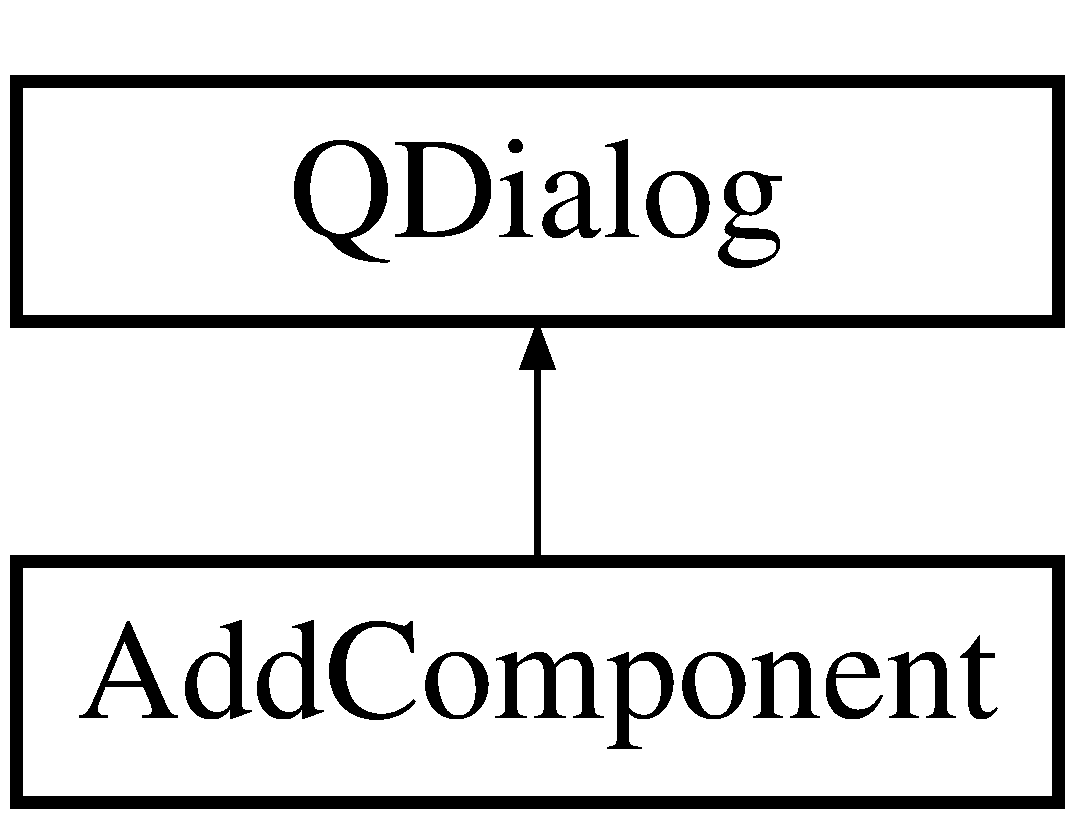
\includegraphics[height=2.000000cm]{classAddComponent}
\end{center}
\end{figure}
\subsection*{Public Member Functions}
\begin{DoxyCompactItemize}
\item 
\hypertarget{classAddComponent_a09f1311751df371815dde94ca52f505e}{{\bfseries Add\-Component} (Q\-Widget $\ast$parent=0)}\label{classAddComponent_a09f1311751df371815dde94ca52f505e}

\end{DoxyCompactItemize}


The documentation for this class was generated from the following files\-:\begin{DoxyCompactItemize}
\item 
addcomponent.\-h\item 
addcomponent.\-cpp\end{DoxyCompactItemize}

\hypertarget{classUi_1_1AddComponent}{\section{Ui\-:\-:Add\-Component Class Reference}
\label{classUi_1_1AddComponent}\index{Ui\-::\-Add\-Component@{Ui\-::\-Add\-Component}}
}
Inheritance diagram for Ui\-:\-:Add\-Component\-:\begin{figure}[H]
\begin{center}
\leavevmode
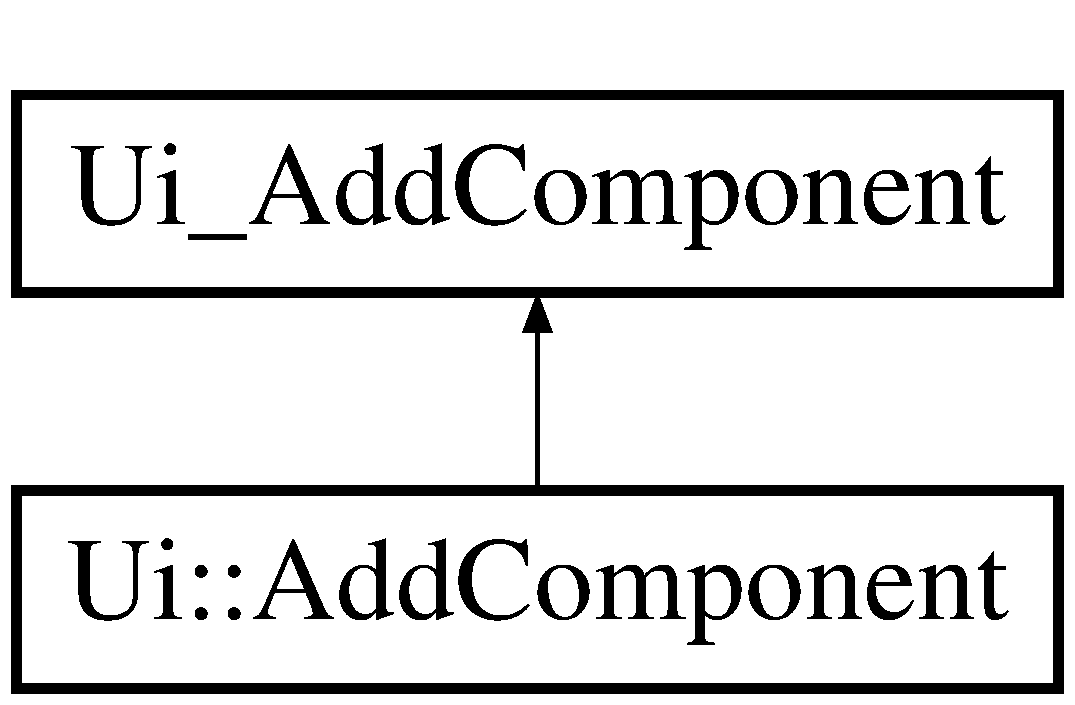
\includegraphics[height=2.000000cm]{classUi_1_1AddComponent}
\end{center}
\end{figure}
\subsection*{Additional Inherited Members}


The documentation for this class was generated from the following file\-:\begin{DoxyCompactItemize}
\item 
ui\-\_\-addcomponent.\-h\end{DoxyCompactItemize}

\hypertarget{classChooseChip}{\section{Choose\-Chip Class Reference}
\label{classChooseChip}\index{Choose\-Chip@{Choose\-Chip}}
}
Inheritance diagram for Choose\-Chip\-:\begin{figure}[H]
\begin{center}
\leavevmode
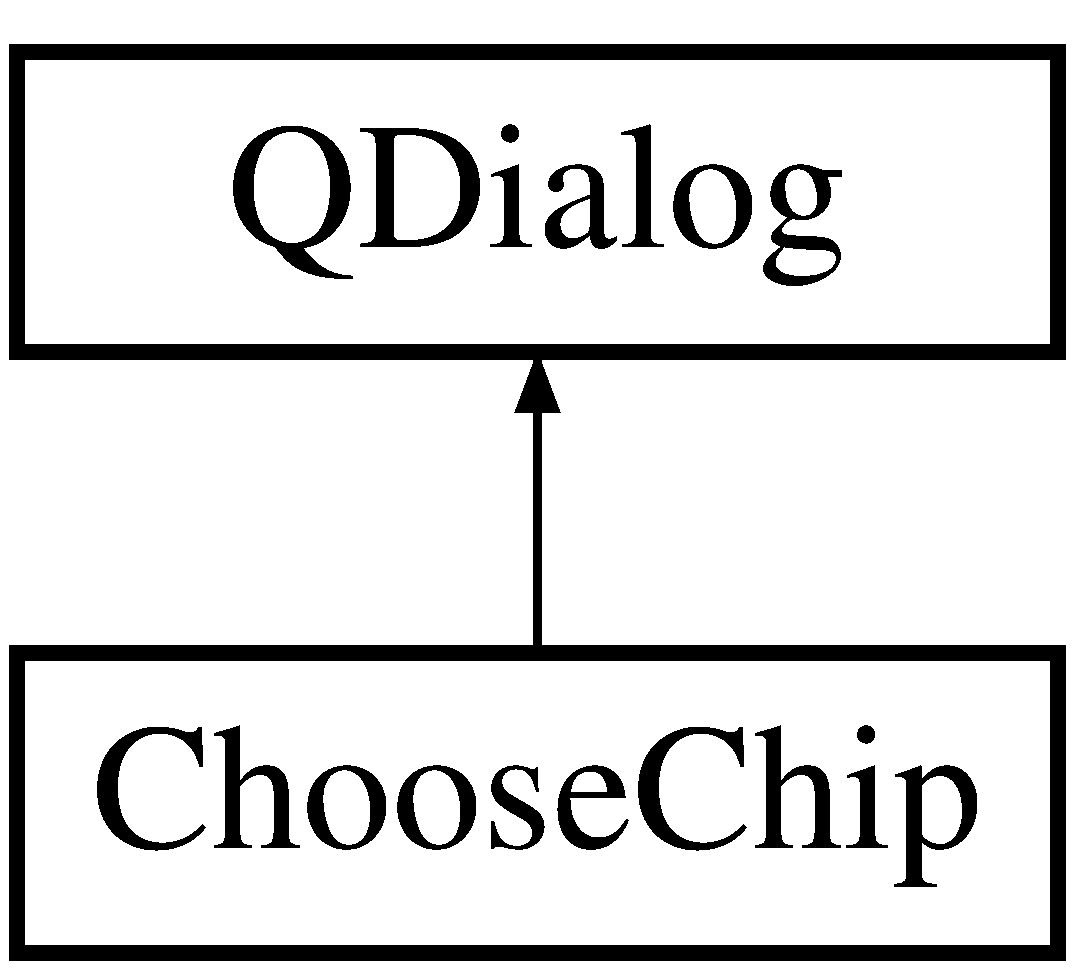
\includegraphics[height=2.000000cm]{classChooseChip}
\end{center}
\end{figure}
\subsection*{Public Member Functions}
\begin{DoxyCompactItemize}
\item 
\hypertarget{classChooseChip_a86433ee7ca248b75b72cdee5c484cc31}{{\bfseries Choose\-Chip} (Q\-Widget $\ast$parent=0)}\label{classChooseChip_a86433ee7ca248b75b72cdee5c484cc31}

\item 
\hypertarget{classChooseChip_a07ac26f7b12d03e8c8dd04f1dfd24c58}{void {\bfseries add\-\_\-chip} (Q\-String chip\-\_\-name)}\label{classChooseChip_a07ac26f7b12d03e8c8dd04f1dfd24c58}

\item 
\hypertarget{classChooseChip_ae34f2a29b05ff8cbb6acc6b72d841370}{void {\bfseries set\-\_\-flash\-\_\-ctx\-\_\-ptr} (fl\-\_\-flashctx\-\_\-t $\ast$$\ast$ctx\-\_\-ptr)}\label{classChooseChip_ae34f2a29b05ff8cbb6acc6b72d841370}

\end{DoxyCompactItemize}


The documentation for this class was generated from the following files\-:\begin{DoxyCompactItemize}
\item 
choosechip.\-h\item 
choosechip.\-cpp\end{DoxyCompactItemize}

\hypertarget{classUi_1_1ChooseChip}{\section{Ui\-:\-:Choose\-Chip Class Reference}
\label{classUi_1_1ChooseChip}\index{Ui\-::\-Choose\-Chip@{Ui\-::\-Choose\-Chip}}
}
Inheritance diagram for Ui\-:\-:Choose\-Chip\-:\begin{figure}[H]
\begin{center}
\leavevmode
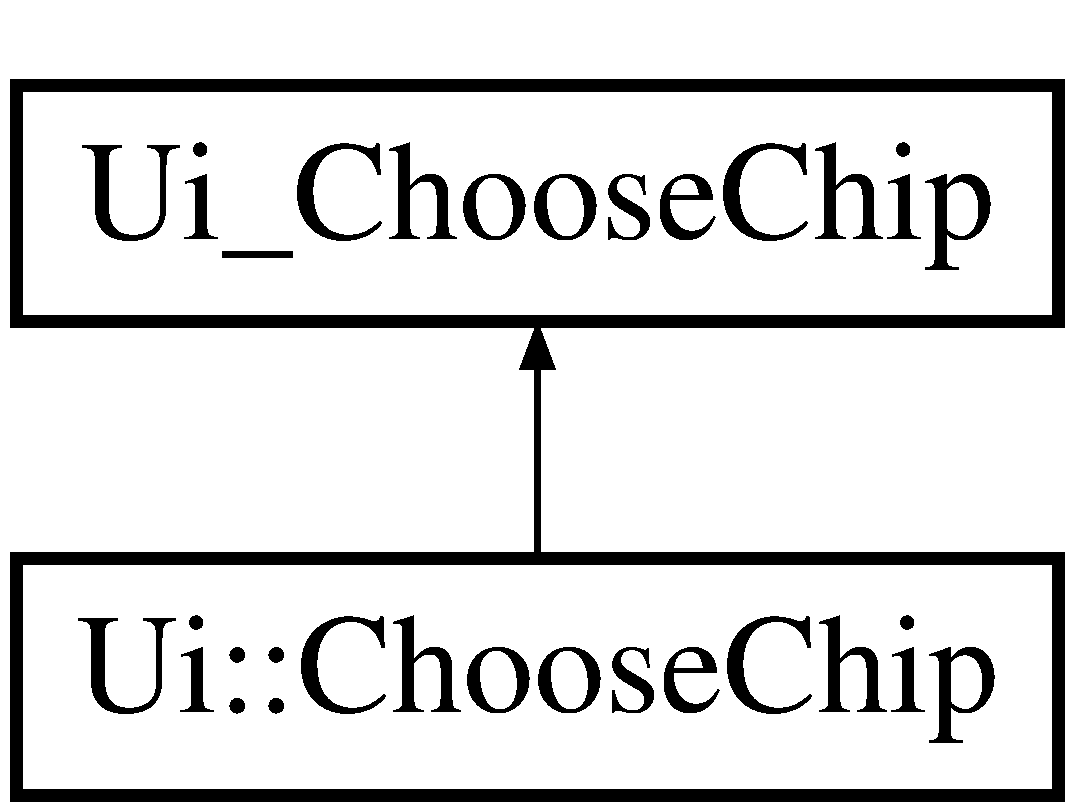
\includegraphics[height=2.000000cm]{classUi_1_1ChooseChip}
\end{center}
\end{figure}
\subsection*{Additional Inherited Members}


The documentation for this class was generated from the following file\-:\begin{DoxyCompactItemize}
\item 
ui\-\_\-choosechip.\-h\end{DoxyCompactItemize}

\hypertarget{classDataGatherer}{\section{Data\-Gatherer Class Reference}
\label{classDataGatherer}\index{Data\-Gatherer@{Data\-Gatherer}}
}
\subsection*{Public Member Functions}
\begin{DoxyCompactItemize}
\item 
\hypertarget{classDataGatherer_a77ded74272e1c80715106081e12b67fb}{R\-E\-T\-\_\-\-V\-A\-L {\bfseries save\-\_\-lspci\-\_\-output} ()}\label{classDataGatherer_a77ded74272e1c80715106081e12b67fb}

\item 
\hypertarget{classDataGatherer_a8ea3c1580b848d09da73fc4422043e0d}{R\-E\-T\-\_\-\-V\-A\-L {\bfseries save\-\_\-edid\-\_\-data} ()}\label{classDataGatherer_a8ea3c1580b848d09da73fc4422043e0d}

\item 
\hypertarget{classDataGatherer_a0f20eb5811ca910ba418bcab7439a99f}{R\-E\-T\-\_\-\-V\-A\-L {\bfseries save\-\_\-dmidecode\-\_\-output} ()}\label{classDataGatherer_a0f20eb5811ca910ba418bcab7439a99f}

\item 
\hypertarget{classDataGatherer_a2183a8a06988a7bcd95170d94d961f85}{R\-E\-T\-\_\-\-V\-A\-L {\bfseries save\-\_\-bios\-\_\-rom\-\_\-factory} (Q\-String save\-\_\-path)}\label{classDataGatherer_a2183a8a06988a7bcd95170d94d961f85}

\item 
\hypertarget{classDataGatherer_a7f6d3d2669450f279064694798912358}{R\-E\-T\-\_\-\-V\-A\-L {\bfseries save\-\_\-bios\-\_\-rom\-\_\-from\-\_\-iomem} ()}\label{classDataGatherer_a7f6d3d2669450f279064694798912358}

\item 
\hypertarget{classDataGatherer_abefb282ecb13454e87779fafe51bfe74}{void {\bfseries extract\-\_\-rom} (Q\-String bios\-\_\-rom\-\_\-path)}\label{classDataGatherer_abefb282ecb13454e87779fafe51bfe74}

\item 
\hypertarget{classDataGatherer_afb8ae017608db79de193dca247b15fc3}{Q\-String {\bfseries get\-\_\-graphic\-\_\-card\-\_\-model} ()}\label{classDataGatherer_afb8ae017608db79de193dca247b15fc3}

\item 
\hypertarget{classDataGatherer_a3e4f5ea1610739e09b433daadc537e3e}{Q\-String {\bfseries get\-\_\-display\-\_\-panel\-\_\-model} ()}\label{classDataGatherer_a3e4f5ea1610739e09b433daadc537e3e}

\item 
\hypertarget{classDataGatherer_a5a2de7e19f4a673e1f88e962f8b32588}{Q\-String {\bfseries get\-\_\-motherboard\-\_\-model} ()}\label{classDataGatherer_a5a2de7e19f4a673e1f88e962f8b32588}

\item 
\hypertarget{classDataGatherer_a5071be7a22f26a1e8c4956fd88756aa6}{R\-E\-T\-\_\-\-V\-A\-L {\bfseries create\-\_\-hardware\-\_\-data\-\_\-archive} ()}\label{classDataGatherer_a5071be7a22f26a1e8c4956fd88756aa6}

\item 
\hypertarget{classDataGatherer_aaea8e9ae23a7f6ea5e0b1b04e9125596}{R\-E\-T\-\_\-\-V\-A\-L {\bfseries unpack\-\_\-hardware\-\_\-data\-\_\-archive} (Q\-String filename)}\label{classDataGatherer_aaea8e9ae23a7f6ea5e0b1b04e9125596}

\end{DoxyCompactItemize}


The documentation for this class was generated from the following files\-:\begin{DoxyCompactItemize}
\item 
datagatherer.\-h\item 
datagatherer.\-cpp\end{DoxyCompactItemize}

\hypertarget{classDeleteComponents}{\section{Delete\-Components Class Reference}
\label{classDeleteComponents}\index{Delete\-Components@{Delete\-Components}}
}
Inheritance diagram for Delete\-Components\-:\begin{figure}[H]
\begin{center}
\leavevmode
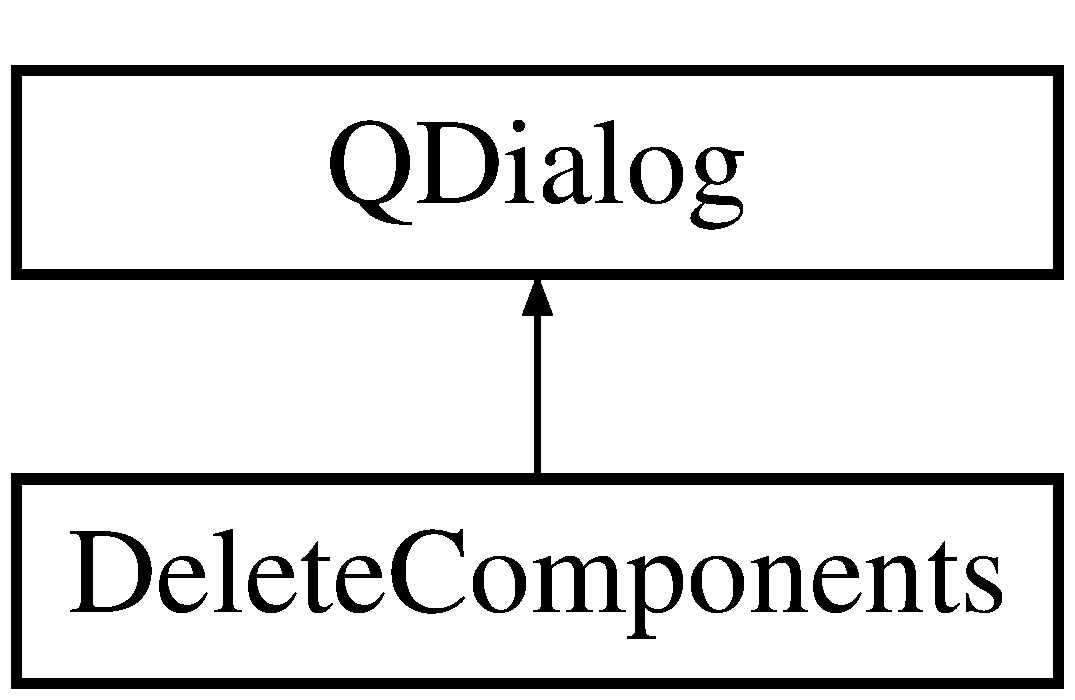
\includegraphics[height=2.000000cm]{classDeleteComponents}
\end{center}
\end{figure}
\subsection*{Public Member Functions}
\begin{DoxyCompactItemize}
\item 
\hypertarget{classDeleteComponents_a27897b1d60d46c4ca576d60d5a71b0ea}{{\bfseries Delete\-Components} (Q\-Widget $\ast$parent=0)}\label{classDeleteComponents_a27897b1d60d46c4ca576d60d5a71b0ea}

\end{DoxyCompactItemize}


The documentation for this class was generated from the following files\-:\begin{DoxyCompactItemize}
\item 
deletecomponents.\-h\item 
deletecomponents.\-cpp\end{DoxyCompactItemize}

\hypertarget{classUi_1_1DeleteComponents}{\section{Ui\-:\-:Delete\-Components Class Reference}
\label{classUi_1_1DeleteComponents}\index{Ui\-::\-Delete\-Components@{Ui\-::\-Delete\-Components}}
}
Inheritance diagram for Ui\-:\-:Delete\-Components\-:\begin{figure}[H]
\begin{center}
\leavevmode
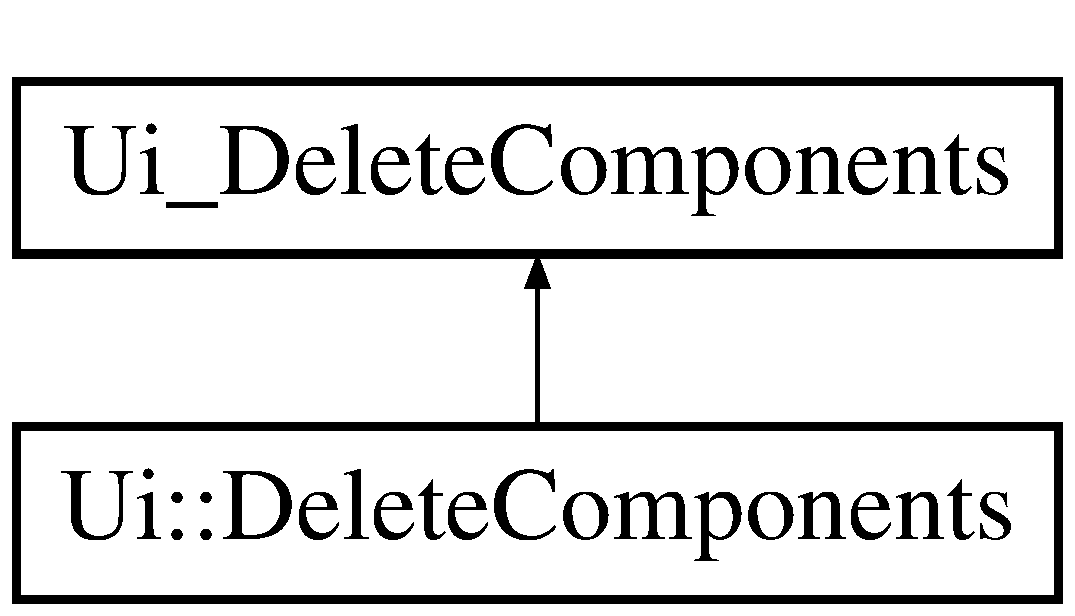
\includegraphics[height=2.000000cm]{classUi_1_1DeleteComponents}
\end{center}
\end{figure}
\subsection*{Additional Inherited Members}


The documentation for this class was generated from the following file\-:\begin{DoxyCompactItemize}
\item 
ui\-\_\-deletecomponents.\-h\end{DoxyCompactItemize}

\hypertarget{classFlasher}{\section{Flasher Class Reference}
\label{classFlasher}\index{Flasher@{Flasher}}
}
\subsection*{Public Member Functions}
\begin{DoxyCompactItemize}
\item 
int \hyperlink{classFlasher_ad41b2dded5ee4422a204470d34785670}{init\-\_\-flashrom} ()
\begin{DoxyCompactList}\small\item\em Initialize flashrom. \end{DoxyCompactList}\item 
int \hyperlink{classFlasher_ae7358cf483ac7c1460e87e0825ac0374}{shutdown\-\_\-flashrom} ()
\begin{DoxyCompactList}\small\item\em Shut down flashrom. \end{DoxyCompactList}\item 
R\-E\-T\-\_\-\-V\-A\-L \hyperlink{classFlasher_ab91e98b53e9d227e6dc973df0e4171de}{probe\-\_\-chip} ()
\begin{DoxyCompactList}\small\item\em Probe for all known chips. \end{DoxyCompactList}\item 
R\-E\-T\-\_\-\-V\-A\-L \hyperlink{classFlasher_aa216f16d2fc46faee3bde07c05d91260}{read\-\_\-chip} (unsigned char $\ast$$\ast$data\-\_\-out, unsigned long $\ast$const chip\-\_\-size)
\begin{DoxyCompactList}\small\item\em Read chip content to array. \end{DoxyCompactList}\item 
R\-E\-T\-\_\-\-V\-A\-L \hyperlink{classFlasher_a333de6a14a78764fddd2ffcdf38980f4}{verify\-\_\-chip} (unsigned char $\ast$$\ast$buffer, unsigned long buffer\-\_\-size)
\begin{DoxyCompactList}\small\item\em Verify chip content with specified data. \end{DoxyCompactList}\item 
R\-E\-T\-\_\-\-V\-A\-L \hyperlink{classFlasher_a0c680da97e2089e9acb5e306b7831a25}{erase\-\_\-chip} ()
\begin{DoxyCompactList}\small\item\em Erase chip contents. \end{DoxyCompactList}\item 
R\-E\-T\-\_\-\-V\-A\-L \hyperlink{classFlasher_af32ba6559c73a8032bbc42b3860a2d1d}{write\-\_\-chip} (unsigned char $\ast$$\ast$data, unsigned long data\-\_\-size)
\begin{DoxyCompactList}\small\item\em Write input data to chip. \end{DoxyCompactList}\item 
\hypertarget{classFlasher_ad3dc0d4e0f4576e0cf998c50d4563d9e}{unsigned long {\bfseries get\-\_\-chip\-\_\-size} ()}\label{classFlasher_ad3dc0d4e0f4576e0cf998c50d4563d9e}

\end{DoxyCompactItemize}


\subsection{Member Function Documentation}
\hypertarget{classFlasher_a0c680da97e2089e9acb5e306b7831a25}{\index{Flasher@{Flasher}!erase\-\_\-chip@{erase\-\_\-chip}}
\index{erase\-\_\-chip@{erase\-\_\-chip}!Flasher@{Flasher}}
\subsubsection[{erase\-\_\-chip}]{\setlength{\rightskip}{0pt plus 5cm}R\-E\-T\-\_\-\-V\-A\-L Flasher\-::erase\-\_\-chip (
\begin{DoxyParamCaption}
{}
\end{DoxyParamCaption}
)}}\label{classFlasher_a0c680da97e2089e9acb5e306b7831a25}


Erase chip contents. 

\begin{DoxyReturn}{Returns}
S\-U\-C\-C\-E\-S\-S -\/ data successfully read 

E\-R\-R\-\_\-\-P\-R\-O\-G\-\_\-\-N\-O\-T\-\_\-\-I\-N\-I\-T -\/ programmer not initialized 

E\-R\-R\-\_\-\-C\-H\-I\-P\-\_\-\-N\-O\-T\-\_\-\-P\-R\-O\-B\-E\-D -\/ chip not probed (no flash context) 
\end{DoxyReturn}
\hypertarget{classFlasher_ad41b2dded5ee4422a204470d34785670}{\index{Flasher@{Flasher}!init\-\_\-flashrom@{init\-\_\-flashrom}}
\index{init\-\_\-flashrom@{init\-\_\-flashrom}!Flasher@{Flasher}}
\subsubsection[{init\-\_\-flashrom}]{\setlength{\rightskip}{0pt plus 5cm}int Flasher\-::init\-\_\-flashrom (
\begin{DoxyParamCaption}
{}
\end{DoxyParamCaption}
)}}\label{classFlasher_ad41b2dded5ee4422a204470d34785670}


Initialize flashrom. 

\begin{DoxyReturn}{Returns}
0 on success 
\end{DoxyReturn}
\hypertarget{classFlasher_ab91e98b53e9d227e6dc973df0e4171de}{\index{Flasher@{Flasher}!probe\-\_\-chip@{probe\-\_\-chip}}
\index{probe\-\_\-chip@{probe\-\_\-chip}!Flasher@{Flasher}}
\subsubsection[{probe\-\_\-chip}]{\setlength{\rightskip}{0pt plus 5cm}R\-E\-T\-\_\-\-V\-A\-L Flasher\-::probe\-\_\-chip (
\begin{DoxyParamCaption}
{}
\end{DoxyParamCaption}
)}}\label{classFlasher_ab91e98b53e9d227e6dc973df0e4171de}


Probe for all known chips. 

Probes for all known chips and if multiple chips are found outputs them in choose dialog

\begin{DoxyReturn}{Returns}
S\-U\-C\-C\-E\-S\-S -\/ chip successfully probed 

E\-R\-R\-\_\-\-P\-R\-O\-G\-\_\-\-N\-O\-T\-\_\-\-I\-N\-I\-T -\/ programmer not initialized 

E\-R\-R\-\_\-\-C\-H\-I\-P\-\_\-\-P\-R\-O\-B\-E\-D -\/ chip has been already probed 

E\-R\-R\-\_\-\-P\-R\-O\-B\-E\-\_\-\-F\-A\-I\-L\-E\-D -\/ probing failed 

U\-N\-K\-N\-O\-W\-N -\/ unknown error 
\end{DoxyReturn}
\hypertarget{classFlasher_aa216f16d2fc46faee3bde07c05d91260}{\index{Flasher@{Flasher}!read\-\_\-chip@{read\-\_\-chip}}
\index{read\-\_\-chip@{read\-\_\-chip}!Flasher@{Flasher}}
\subsubsection[{read\-\_\-chip}]{\setlength{\rightskip}{0pt plus 5cm}R\-E\-T\-\_\-\-V\-A\-L Flasher\-::read\-\_\-chip (
\begin{DoxyParamCaption}
\item[{unsigned char $\ast$$\ast$}]{data\-\_\-out, }
\item[{unsigned long $\ast$const}]{chip\-\_\-size}
\end{DoxyParamCaption}
)}}\label{classFlasher_aa216f16d2fc46faee3bde07c05d91260}


Read chip content to array. 

Reads chip content, then allocates memory and fills it with read data


\begin{DoxyParams}{Parameters}
{\em data\-\_\-out} & \mbox{[}out\mbox{]} pointer to read data \\
\hline
{\em chip\-\_\-size} & \mbox{[}out\mbox{]} size of chip in bytes \\
\hline
\end{DoxyParams}
\begin{DoxyReturn}{Returns}
S\-U\-C\-C\-E\-S\-S -\/ data successfully read 

E\-R\-R\-\_\-\-P\-R\-O\-G\-\_\-\-N\-O\-T\-\_\-\-I\-N\-I\-T -\/ programmer not initialized 

E\-R\-R\-\_\-\-C\-H\-I\-P\-\_\-\-N\-O\-T\-\_\-\-P\-R\-O\-B\-E\-D -\/ chip not probed (no flash context) 

E\-R\-R\-\_\-\-M\-E\-M\-\_\-\-A\-L\-L\-O\-C -\/ memory allocation failed 

U\-N\-K\-N\-O\-W\-N -\/ unknown error 
\end{DoxyReturn}
\hypertarget{classFlasher_ae7358cf483ac7c1460e87e0825ac0374}{\index{Flasher@{Flasher}!shutdown\-\_\-flashrom@{shutdown\-\_\-flashrom}}
\index{shutdown\-\_\-flashrom@{shutdown\-\_\-flashrom}!Flasher@{Flasher}}
\subsubsection[{shutdown\-\_\-flashrom}]{\setlength{\rightskip}{0pt plus 5cm}int Flasher\-::shutdown\-\_\-flashrom (
\begin{DoxyParamCaption}
{}
\end{DoxyParamCaption}
)}}\label{classFlasher_ae7358cf483ac7c1460e87e0825ac0374}


Shut down flashrom. 

\begin{DoxyReturn}{Returns}
0 on success 
\end{DoxyReturn}
\hypertarget{classFlasher_a333de6a14a78764fddd2ffcdf38980f4}{\index{Flasher@{Flasher}!verify\-\_\-chip@{verify\-\_\-chip}}
\index{verify\-\_\-chip@{verify\-\_\-chip}!Flasher@{Flasher}}
\subsubsection[{verify\-\_\-chip}]{\setlength{\rightskip}{0pt plus 5cm}R\-E\-T\-\_\-\-V\-A\-L Flasher\-::verify\-\_\-chip (
\begin{DoxyParamCaption}
\item[{unsigned char $\ast$$\ast$}]{buffer, }
\item[{unsigned long}]{buffer\-\_\-size}
\end{DoxyParamCaption}
)}}\label{classFlasher_a333de6a14a78764fddd2ffcdf38980f4}


Verify chip content with specified data. 


\begin{DoxyParams}{Parameters}
{\em buffer} & \mbox{[}in\mbox{]} pointer to input data \\
\hline
{\em buffer\-\_\-size} & \mbox{[}in\mbox{]} size of pointed data in bytes \\
\hline
\end{DoxyParams}
\begin{DoxyReturn}{Returns}
S\-U\-C\-C\-E\-S\-S -\/ data successfully read 

E\-R\-R\-\_\-\-P\-R\-O\-G\-\_\-\-N\-O\-T\-\_\-\-I\-N\-I\-T -\/ programmer not initialized 

E\-R\-R\-\_\-\-C\-H\-I\-P\-\_\-\-N\-O\-T\-\_\-\-P\-R\-O\-B\-E\-D -\/ chip not probed (no flash context) 

E\-R\-R\-\_\-\-C\-H\-I\-P\-\_\-\-N\-O\-T\-\_\-\-V\-E\-R\-I\-F\-I\-E\-D -\/ chip contents is not consistent with input data 

E\-R\-R\-\_\-\-B\-U\-F\-\_\-\-S\-I\-Z\-E\-\_\-\-D\-I\-F\-F -\/ size of input data is not consistent with size of a chip 

U\-N\-K\-N\-O\-W\-N -\/ unknown error 
\end{DoxyReturn}
\hypertarget{classFlasher_af32ba6559c73a8032bbc42b3860a2d1d}{\index{Flasher@{Flasher}!write\-\_\-chip@{write\-\_\-chip}}
\index{write\-\_\-chip@{write\-\_\-chip}!Flasher@{Flasher}}
\subsubsection[{write\-\_\-chip}]{\setlength{\rightskip}{0pt plus 5cm}R\-E\-T\-\_\-\-V\-A\-L Flasher\-::write\-\_\-chip (
\begin{DoxyParamCaption}
\item[{unsigned char $\ast$$\ast$}]{data, }
\item[{unsigned long}]{data\-\_\-size}
\end{DoxyParamCaption}
)}}\label{classFlasher_af32ba6559c73a8032bbc42b3860a2d1d}


Write input data to chip. 


\begin{DoxyParams}{Parameters}
{\em data} & \mbox{[}in\mbox{]} pointer to input data \\
\hline
{\em data\-\_\-size} & \mbox{[}in\mbox{]} size of pointed data in bytes \\
\hline
\end{DoxyParams}
\begin{DoxyReturn}{Returns}
S\-U\-C\-C\-E\-S\-S -\/ data successfully read 

E\-R\-R\-\_\-\-P\-R\-O\-G\-\_\-\-N\-O\-T\-\_\-\-I\-N\-I\-T -\/ programmer not initialized 

E\-R\-R\-\_\-\-C\-H\-I\-P\-\_\-\-N\-O\-T\-\_\-\-P\-R\-O\-B\-E\-D -\/ chip not probed (no flash context) 

E\-R\-R\-\_\-\-W\-R\-I\-T\-E\-\_\-\-F\-A\-I\-L\-E\-D -\/ write to chip failed 

E\-R\-R\-\_\-\-B\-U\-F\-\_\-\-S\-I\-Z\-E\-\_\-\-D\-I\-F\-F -\/ size of input data is not consistent with size of a chip 

U\-N\-K\-N\-O\-W\-N -\/ unknown error 
\end{DoxyReturn}


The documentation for this class was generated from the following files\-:\begin{DoxyCompactItemize}
\item 
flasher.\-h\item 
flasher.\-cpp\end{DoxyCompactItemize}

\hypertarget{classInfoDialog}{\section{Info\-Dialog Class Reference}
\label{classInfoDialog}\index{Info\-Dialog@{Info\-Dialog}}
}
Inheritance diagram for Info\-Dialog\-:\begin{figure}[H]
\begin{center}
\leavevmode
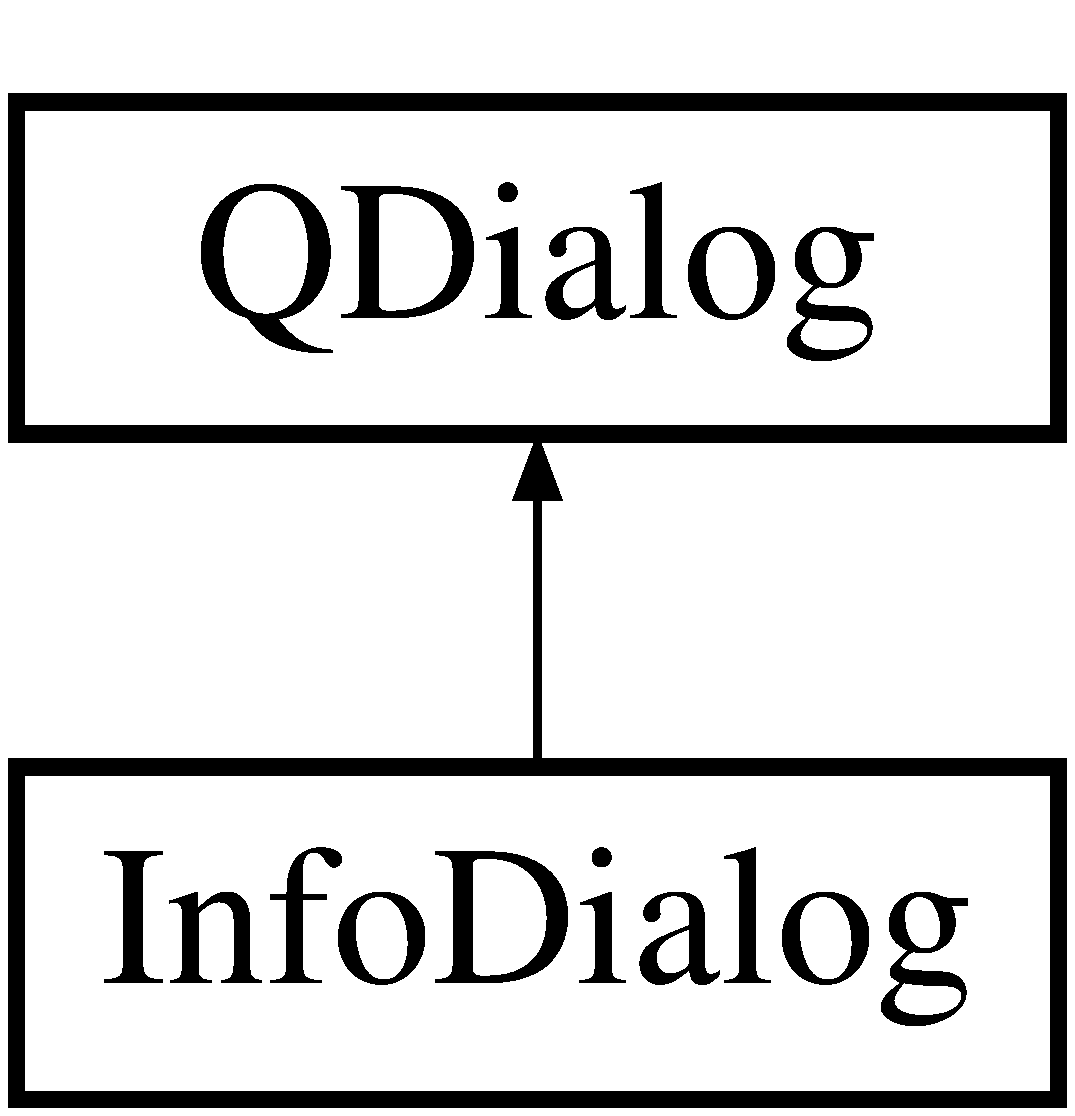
\includegraphics[height=2.000000cm]{classInfoDialog}
\end{center}
\end{figure}
\subsection*{Public Member Functions}
\begin{DoxyCompactItemize}
\item 
\hypertarget{classInfoDialog_a446583cff8652d633f59db711bad2edc}{{\bfseries Info\-Dialog} (Q\-Widget $\ast$parent=0)}\label{classInfoDialog_a446583cff8652d633f59db711bad2edc}

\item 
\hypertarget{classInfoDialog_aec99044be3072eddb6a84fc8073063fb}{void {\bfseries show\-\_\-message} (R\-E\-T\-\_\-\-V\-A\-L ret\-\_\-val)}\label{classInfoDialog_aec99044be3072eddb6a84fc8073063fb}

\end{DoxyCompactItemize}


The documentation for this class was generated from the following files\-:\begin{DoxyCompactItemize}
\item 
infodialog.\-h\item 
infodialog.\-cpp\end{DoxyCompactItemize}

\hypertarget{classUi_1_1InfoDialog}{\section{Ui\-:\-:Info\-Dialog Class Reference}
\label{classUi_1_1InfoDialog}\index{Ui\-::\-Info\-Dialog@{Ui\-::\-Info\-Dialog}}
}
Inheritance diagram for Ui\-:\-:Info\-Dialog\-:\begin{figure}[H]
\begin{center}
\leavevmode
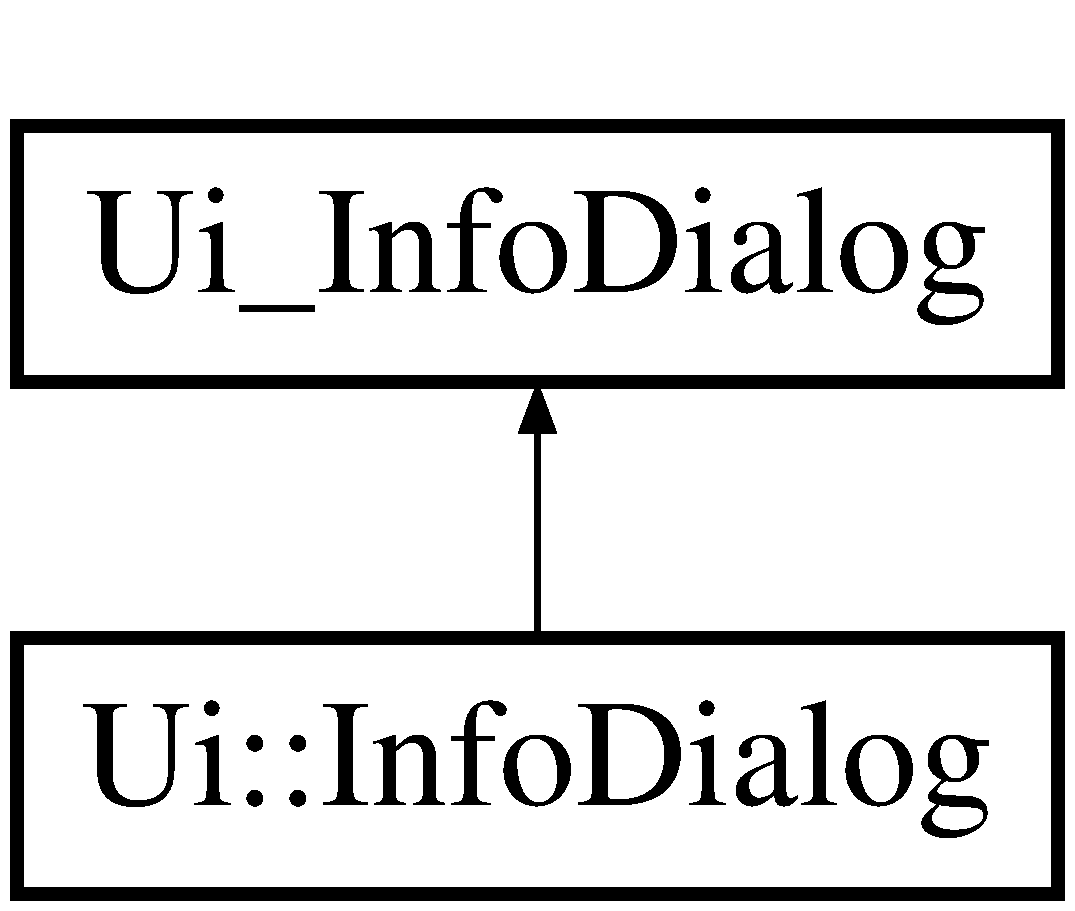
\includegraphics[height=2.000000cm]{classUi_1_1InfoDialog}
\end{center}
\end{figure}
\subsection*{Additional Inherited Members}


The documentation for this class was generated from the following file\-:\begin{DoxyCompactItemize}
\item 
ui\-\_\-infodialog.\-h\end{DoxyCompactItemize}

\hypertarget{classMainWindow}{\section{Main\-Window Class Reference}
\label{classMainWindow}\index{Main\-Window@{Main\-Window}}
}
Inheritance diagram for Main\-Window\-:\begin{figure}[H]
\begin{center}
\leavevmode
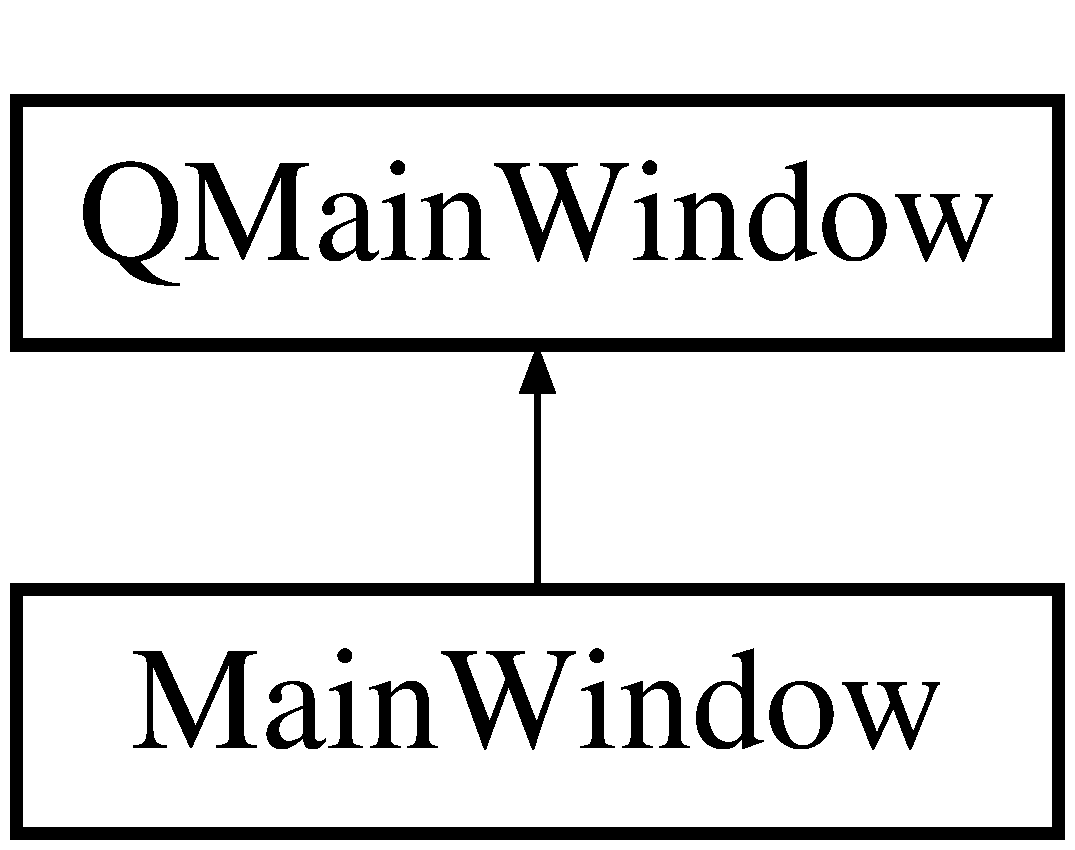
\includegraphics[height=2.000000cm]{classMainWindow}
\end{center}
\end{figure}
\subsection*{Public Member Functions}
\begin{DoxyCompactItemize}
\item 
\hypertarget{classMainWindow_a8b244be8b7b7db1b08de2a2acb9409db}{{\bfseries Main\-Window} (Q\-Widget $\ast$parent=0)}\label{classMainWindow_a8b244be8b7b7db1b08de2a2acb9409db}

\item 
\hypertarget{classMainWindow_a7aa165ddf55717d85ab6f744f63c8795}{Q\-String {\bfseries get\-\_\-cbfs\-\_\-rom\-\_\-path} ()}\label{classMainWindow_a7aa165ddf55717d85ab6f744f63c8795}

\end{DoxyCompactItemize}
\subsection*{Public Attributes}
\begin{DoxyCompactItemize}
\item 
\hypertarget{classMainWindow_a35466a70ed47252a0191168126a352a5}{\hyperlink{classUi_1_1MainWindow}{Ui\-::\-Main\-Window} $\ast$ {\bfseries ui}}\label{classMainWindow_a35466a70ed47252a0191168126a352a5}

\item 
\hypertarget{classMainWindow_acb081a83000d665b349943e012e14c67}{Q\-Text\-Edit $\ast$ {\bfseries active\-\_\-log\-\_\-out}}\label{classMainWindow_acb081a83000d665b349943e012e14c67}

\item 
\hypertarget{classMainWindow_a898a7f35b61cbb1668be8ab027ee6c87}{Q\-String {\bfseries chip\-\_\-name}}\label{classMainWindow_a898a7f35b61cbb1668be8ab027ee6c87}

\item 
\hypertarget{classMainWindow_af3641fe0d6d71b6fe3ada1a7fd9f0abe}{Q\-String {\bfseries coreboot\-\_\-dir}}\label{classMainWindow_af3641fe0d6d71b6fe3ada1a7fd9f0abe}

\item 
\hypertarget{classMainWindow_aa9b9e4aa3b2225b372c723f900fd4840}{Q\-String {\bfseries factory\-\_\-bios\-\_\-dir}}\label{classMainWindow_aa9b9e4aa3b2225b372c723f900fd4840}

\item 
\hypertarget{classMainWindow_afe8040a491f4140c36c4d1cca2a63390}{bool {\bfseries chip\-\_\-found}}\label{classMainWindow_afe8040a491f4140c36c4d1cca2a63390}

\item 
\hypertarget{classMainWindow_ade45675d9c29a12f3891c0e5ffb6b520}{bool {\bfseries programmer\-\_\-initialized}}\label{classMainWindow_ade45675d9c29a12f3891c0e5ffb6b520}

\item 
\hypertarget{classMainWindow_add53793006fe49da98302a2f0df4f34f}{\hyperlink{classInfoDialog}{Info\-Dialog} $\ast$ {\bfseries info\-\_\-dialog}}\label{classMainWindow_add53793006fe49da98302a2f0df4f34f}

\end{DoxyCompactItemize}


The documentation for this class was generated from the following files\-:\begin{DoxyCompactItemize}
\item 
mainwindow.\-h\item 
mainwindow.\-cpp\end{DoxyCompactItemize}

\hypertarget{classUi_1_1MainWindow}{\section{Ui\-:\-:Main\-Window Class Reference}
\label{classUi_1_1MainWindow}\index{Ui\-::\-Main\-Window@{Ui\-::\-Main\-Window}}
}
Inheritance diagram for Ui\-:\-:Main\-Window\-:\begin{figure}[H]
\begin{center}
\leavevmode
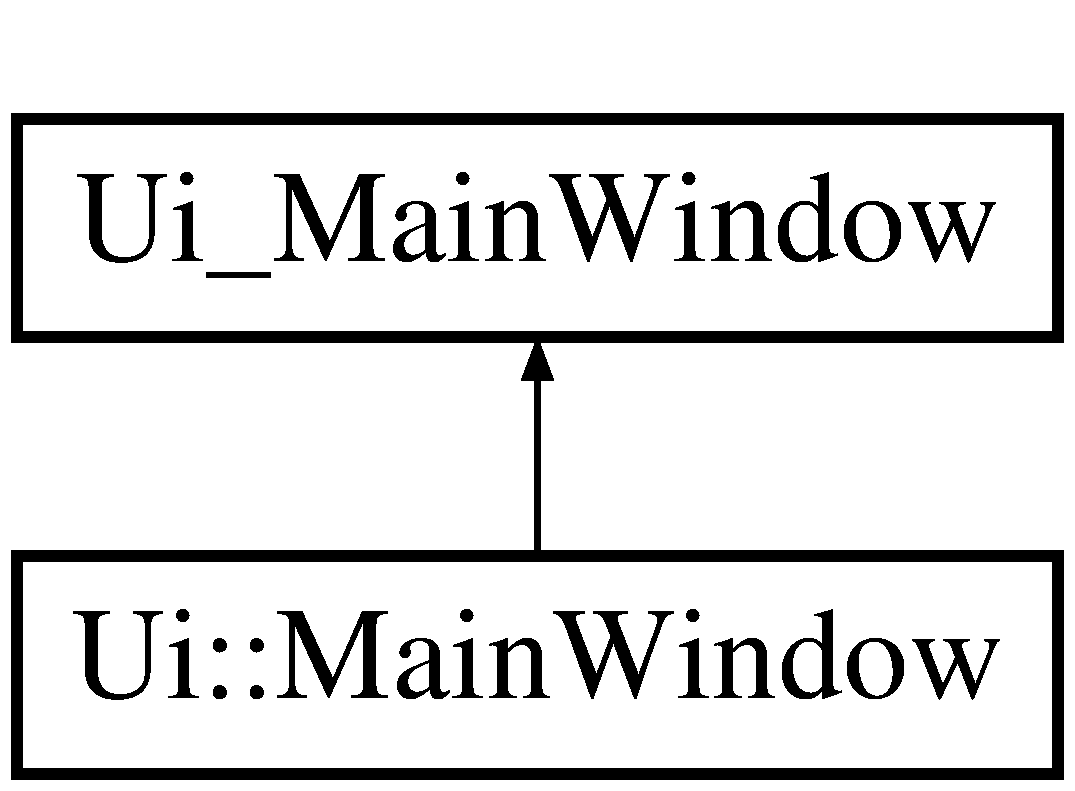
\includegraphics[height=2.000000cm]{classUi_1_1MainWindow}
\end{center}
\end{figure}
\subsection*{Additional Inherited Members}


The documentation for this class was generated from the following file\-:\begin{DoxyCompactItemize}
\item 
ui\-\_\-mainwindow.\-h\end{DoxyCompactItemize}

\hypertarget{classMultiSortFilterModel}{\section{Multi\-Sort\-Filter\-Model Class Reference}
\label{classMultiSortFilterModel}\index{Multi\-Sort\-Filter\-Model@{Multi\-Sort\-Filter\-Model}}
}
Inheritance diagram for Multi\-Sort\-Filter\-Model\-:\begin{figure}[H]
\begin{center}
\leavevmode
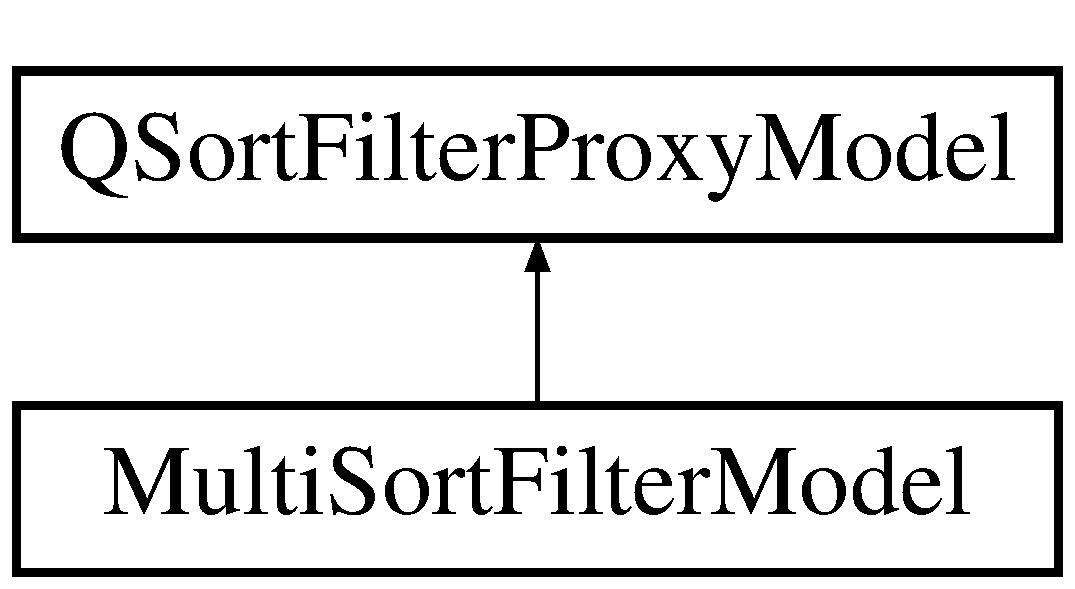
\includegraphics[height=2.000000cm]{classMultiSortFilterModel}
\end{center}
\end{figure}
\subsection*{Public Member Functions}
\begin{DoxyCompactItemize}
\item 
\hypertarget{classMultiSortFilterModel_a699c545b421837b006e064ca6be97016}{{\bfseries Multi\-Sort\-Filter\-Model} (Q\-Object $\ast$parent=0)}\label{classMultiSortFilterModel_a699c545b421837b006e064ca6be97016}

\item 
\hypertarget{classMultiSortFilterModel_a66d2fe690a6603dd520c38a13f2b6a9a}{void {\bfseries set\-Filter\-Key\-Columns} (const Q\-List$<$ qint32 $>$ \&filter\-Columns)}\label{classMultiSortFilterModel_a66d2fe690a6603dd520c38a13f2b6a9a}

\item 
\hypertarget{classMultiSortFilterModel_a924f1e5389e8045f072b7c8eec79b97b}{void {\bfseries set\-Filter} (qint32 column, const Q\-String \&pattern)}\label{classMultiSortFilterModel_a924f1e5389e8045f072b7c8eec79b97b}

\end{DoxyCompactItemize}
\subsection*{Protected Member Functions}
\begin{DoxyCompactItemize}
\item 
\hypertarget{classMultiSortFilterModel_a308fb74918e50bba787fbcb82fb04f91}{bool {\bfseries filter\-Accepts\-Row} (int source\-Row, const Q\-Model\-Index \&source\-Parent) const }\label{classMultiSortFilterModel_a308fb74918e50bba787fbcb82fb04f91}

\end{DoxyCompactItemize}


The documentation for this class was generated from the following files\-:\begin{DoxyCompactItemize}
\item 
multisortfiltermodel.\-h\item 
multisortfiltermodel.\-cpp\end{DoxyCompactItemize}

\hypertarget{classUi_1_1Preferences}{\section{Ui\-:\-:Preferences Class Reference}
\label{classUi_1_1Preferences}\index{Ui\-::\-Preferences@{Ui\-::\-Preferences}}
}
Inheritance diagram for Ui\-:\-:Preferences\-:\begin{figure}[H]
\begin{center}
\leavevmode
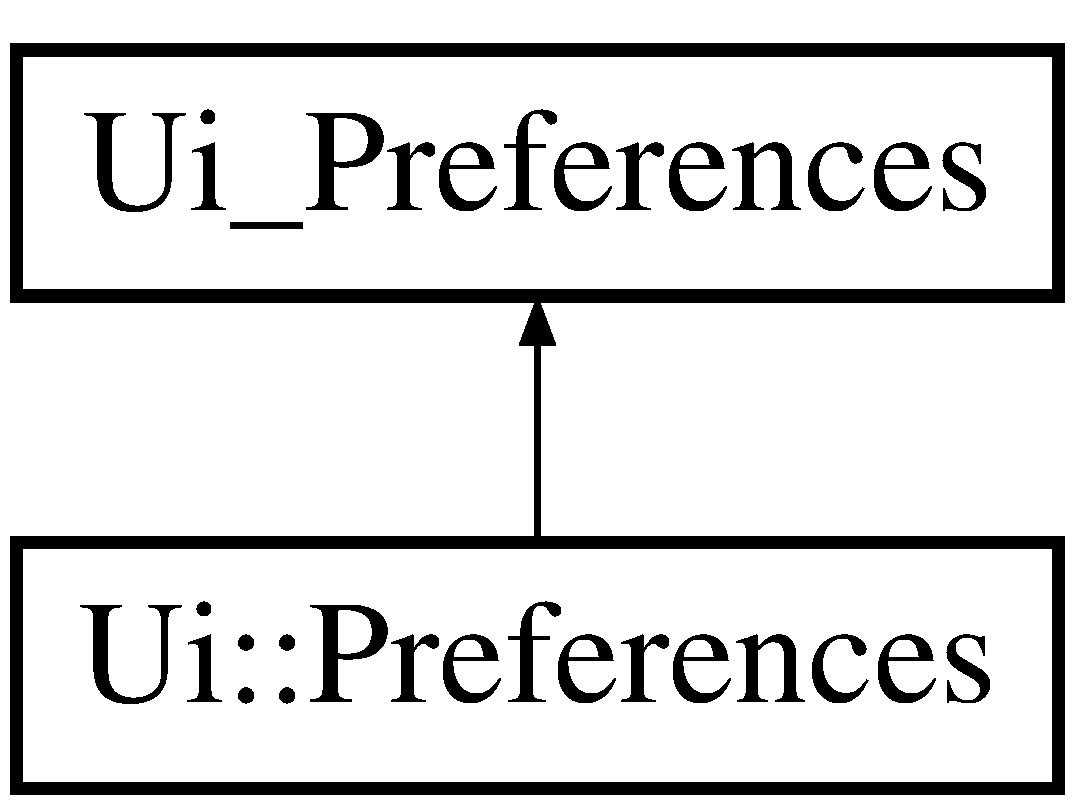
\includegraphics[height=2.000000cm]{classUi_1_1Preferences}
\end{center}
\end{figure}
\subsection*{Additional Inherited Members}


The documentation for this class was generated from the following file\-:\begin{DoxyCompactItemize}
\item 
ui\-\_\-preferences.\-h\end{DoxyCompactItemize}

\hypertarget{classPreferences}{\section{Preferences Class Reference}
\label{classPreferences}\index{Preferences@{Preferences}}
}
Inheritance diagram for Preferences\-:\begin{figure}[H]
\begin{center}
\leavevmode
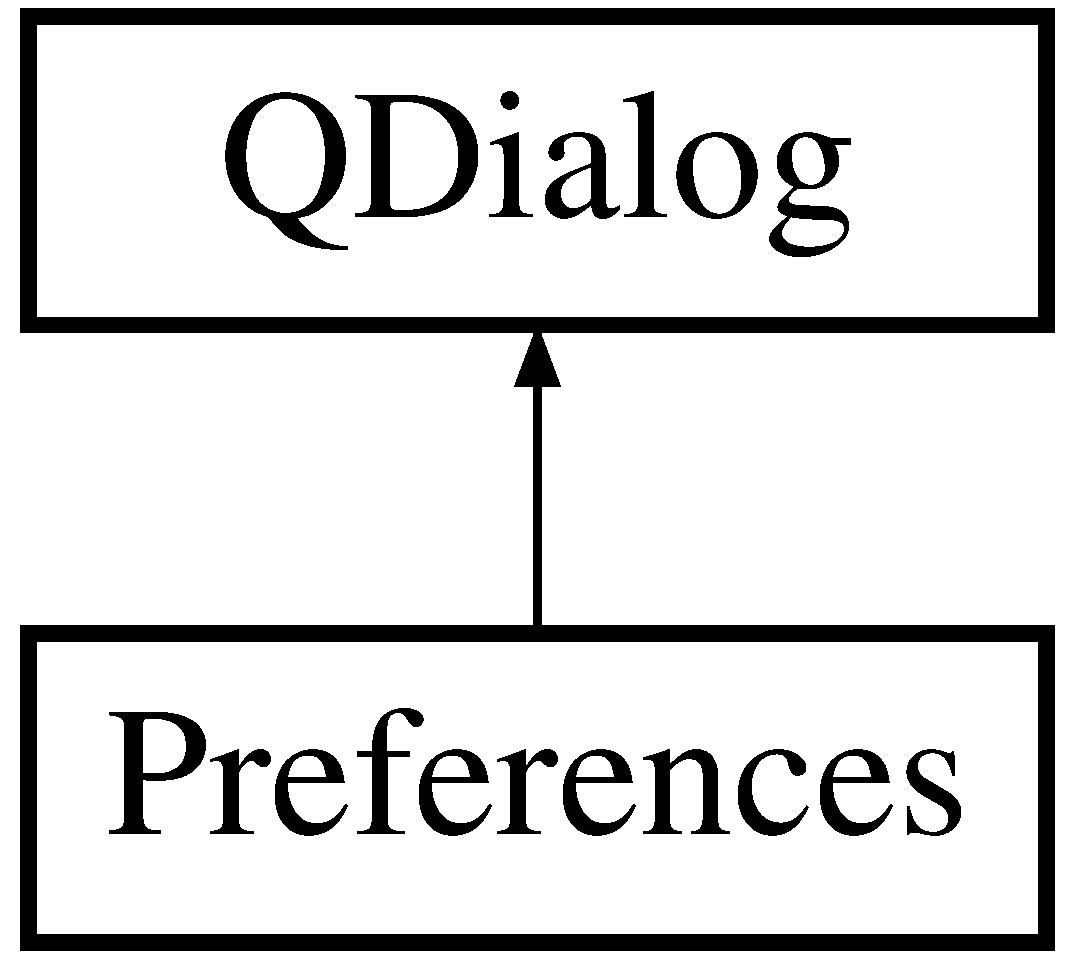
\includegraphics[height=2.000000cm]{classPreferences}
\end{center}
\end{figure}
\subsection*{Public Member Functions}
\begin{DoxyCompactItemize}
\item 
\hypertarget{classPreferences_a3fc460c1a11115945b78b2d35d7ade00}{{\bfseries Preferences} (Q\-Widget $\ast$parent=0)}\label{classPreferences_a3fc460c1a11115945b78b2d35d7ade00}

\end{DoxyCompactItemize}


The documentation for this class was generated from the following files\-:\begin{DoxyCompactItemize}
\item 
preferences.\-h\item 
preferences.\-cpp\end{DoxyCompactItemize}

\hypertarget{structqt__meta__stringdata__About__t}{\section{qt\-\_\-meta\-\_\-stringdata\-\_\-\-About\-\_\-t Struct Reference}
\label{structqt__meta__stringdata__About__t}\index{qt\-\_\-meta\-\_\-stringdata\-\_\-\-About\-\_\-t@{qt\-\_\-meta\-\_\-stringdata\-\_\-\-About\-\_\-t}}
}
\subsection*{Public Attributes}
\begin{DoxyCompactItemize}
\item 
\hypertarget{structqt__meta__stringdata__About__t_aad871b20972058ad4ed0f071f3c4cdc2}{Q\-Byte\-Array\-Data {\bfseries data} \mbox{[}3\mbox{]}}\label{structqt__meta__stringdata__About__t_aad871b20972058ad4ed0f071f3c4cdc2}

\item 
\hypertarget{structqt__meta__stringdata__About__t_a5516a7089c28c3c85a299bf145958a14}{char {\bfseries stringdata} \mbox{[}32\mbox{]}}\label{structqt__meta__stringdata__About__t_a5516a7089c28c3c85a299bf145958a14}

\end{DoxyCompactItemize}


The documentation for this struct was generated from the following file\-:\begin{DoxyCompactItemize}
\item 
moc\-\_\-about.\-cpp\end{DoxyCompactItemize}

\hypertarget{structqt__meta__stringdata__AddComponent__t}{\section{qt\-\_\-meta\-\_\-stringdata\-\_\-\-Add\-Component\-\_\-t Struct Reference}
\label{structqt__meta__stringdata__AddComponent__t}\index{qt\-\_\-meta\-\_\-stringdata\-\_\-\-Add\-Component\-\_\-t@{qt\-\_\-meta\-\_\-stringdata\-\_\-\-Add\-Component\-\_\-t}}
}
\subsection*{Public Attributes}
\begin{DoxyCompactItemize}
\item 
\hypertarget{structqt__meta__stringdata__AddComponent__t_ae3fc0f4a6112d54b8aada2f90bbc1f51}{Q\-Byte\-Array\-Data {\bfseries data} \mbox{[}4\mbox{]}}\label{structqt__meta__stringdata__AddComponent__t_ae3fc0f4a6112d54b8aada2f90bbc1f51}

\item 
\hypertarget{structqt__meta__stringdata__AddComponent__t_ad7b2110ba94f0cb62946737463df538f}{char {\bfseries stringdata} \mbox{[}68\mbox{]}}\label{structqt__meta__stringdata__AddComponent__t_ad7b2110ba94f0cb62946737463df538f}

\end{DoxyCompactItemize}


The documentation for this struct was generated from the following file\-:\begin{DoxyCompactItemize}
\item 
moc\-\_\-addcomponent.\-cpp\end{DoxyCompactItemize}

\hypertarget{structqt__meta__stringdata__ChooseChip__t}{\section{qt\-\_\-meta\-\_\-stringdata\-\_\-\-Choose\-Chip\-\_\-t Struct Reference}
\label{structqt__meta__stringdata__ChooseChip__t}\index{qt\-\_\-meta\-\_\-stringdata\-\_\-\-Choose\-Chip\-\_\-t@{qt\-\_\-meta\-\_\-stringdata\-\_\-\-Choose\-Chip\-\_\-t}}
}
\subsection*{Public Attributes}
\begin{DoxyCompactItemize}
\item 
\hypertarget{structqt__meta__stringdata__ChooseChip__t_a4e575ad4e41f87878c4772c85026e8c0}{Q\-Byte\-Array\-Data {\bfseries data} \mbox{[}3\mbox{]}}\label{structqt__meta__stringdata__ChooseChip__t_a4e575ad4e41f87878c4772c85026e8c0}

\item 
\hypertarget{structqt__meta__stringdata__ChooseChip__t_ae32f0f6157995ecc3b9d42511167006e}{char {\bfseries stringdata} \mbox{[}33\mbox{]}}\label{structqt__meta__stringdata__ChooseChip__t_ae32f0f6157995ecc3b9d42511167006e}

\end{DoxyCompactItemize}


The documentation for this struct was generated from the following file\-:\begin{DoxyCompactItemize}
\item 
moc\-\_\-choosechip.\-cpp\end{DoxyCompactItemize}

\hypertarget{structqt__meta__stringdata__DeleteComponents__t}{\section{qt\-\_\-meta\-\_\-stringdata\-\_\-\-Delete\-Components\-\_\-t Struct Reference}
\label{structqt__meta__stringdata__DeleteComponents__t}\index{qt\-\_\-meta\-\_\-stringdata\-\_\-\-Delete\-Components\-\_\-t@{qt\-\_\-meta\-\_\-stringdata\-\_\-\-Delete\-Components\-\_\-t}}
}
\subsection*{Public Attributes}
\begin{DoxyCompactItemize}
\item 
\hypertarget{structqt__meta__stringdata__DeleteComponents__t_af6c97bc53324cc1645c2cb3af2b76440}{Q\-Byte\-Array\-Data {\bfseries data} \mbox{[}3\mbox{]}}\label{structqt__meta__stringdata__DeleteComponents__t_af6c97bc53324cc1645c2cb3af2b76440}

\item 
\hypertarget{structqt__meta__stringdata__DeleteComponents__t_a78d3eb4df0fc087d4b3e953fe71815f6}{char {\bfseries stringdata} \mbox{[}43\mbox{]}}\label{structqt__meta__stringdata__DeleteComponents__t_a78d3eb4df0fc087d4b3e953fe71815f6}

\end{DoxyCompactItemize}


The documentation for this struct was generated from the following file\-:\begin{DoxyCompactItemize}
\item 
moc\-\_\-deletecomponents.\-cpp\end{DoxyCompactItemize}

\hypertarget{structqt__meta__stringdata__InfoDialog__t}{\section{qt\-\_\-meta\-\_\-stringdata\-\_\-\-Info\-Dialog\-\_\-t Struct Reference}
\label{structqt__meta__stringdata__InfoDialog__t}\index{qt\-\_\-meta\-\_\-stringdata\-\_\-\-Info\-Dialog\-\_\-t@{qt\-\_\-meta\-\_\-stringdata\-\_\-\-Info\-Dialog\-\_\-t}}
}
\subsection*{Public Attributes}
\begin{DoxyCompactItemize}
\item 
\hypertarget{structqt__meta__stringdata__InfoDialog__t_a0ec892214de5cb1b320e4276cb37aae9}{Q\-Byte\-Array\-Data {\bfseries data} \mbox{[}3\mbox{]}}\label{structqt__meta__stringdata__InfoDialog__t_a0ec892214de5cb1b320e4276cb37aae9}

\item 
\hypertarget{structqt__meta__stringdata__InfoDialog__t_a7415576065e3579a5a8ea8f5eb3cb3e9}{char {\bfseries stringdata} \mbox{[}28\mbox{]}}\label{structqt__meta__stringdata__InfoDialog__t_a7415576065e3579a5a8ea8f5eb3cb3e9}

\end{DoxyCompactItemize}


The documentation for this struct was generated from the following file\-:\begin{DoxyCompactItemize}
\item 
moc\-\_\-infodialog.\-cpp\end{DoxyCompactItemize}

\hypertarget{structqt__meta__stringdata__MainWindow__t}{\section{qt\-\_\-meta\-\_\-stringdata\-\_\-\-Main\-Window\-\_\-t Struct Reference}
\label{structqt__meta__stringdata__MainWindow__t}\index{qt\-\_\-meta\-\_\-stringdata\-\_\-\-Main\-Window\-\_\-t@{qt\-\_\-meta\-\_\-stringdata\-\_\-\-Main\-Window\-\_\-t}}
}
\subsection*{Public Attributes}
\begin{DoxyCompactItemize}
\item 
\hypertarget{structqt__meta__stringdata__MainWindow__t_a48f255bc47fc5d9f118e582b8447d10a}{Q\-Byte\-Array\-Data {\bfseries data} \mbox{[}26\mbox{]}}\label{structqt__meta__stringdata__MainWindow__t_a48f255bc47fc5d9f118e582b8447d10a}

\item 
\hypertarget{structqt__meta__stringdata__MainWindow__t_a8a8b1caf3c4a7f2c225e54bf6e887a72}{char {\bfseries stringdata} \mbox{[}586\mbox{]}}\label{structqt__meta__stringdata__MainWindow__t_a8a8b1caf3c4a7f2c225e54bf6e887a72}

\end{DoxyCompactItemize}


The documentation for this struct was generated from the following file\-:\begin{DoxyCompactItemize}
\item 
moc\-\_\-mainwindow.\-cpp\end{DoxyCompactItemize}

\hypertarget{structqt__meta__stringdata__MultiSortFilterModel__t}{\section{qt\-\_\-meta\-\_\-stringdata\-\_\-\-Multi\-Sort\-Filter\-Model\-\_\-t Struct Reference}
\label{structqt__meta__stringdata__MultiSortFilterModel__t}\index{qt\-\_\-meta\-\_\-stringdata\-\_\-\-Multi\-Sort\-Filter\-Model\-\_\-t@{qt\-\_\-meta\-\_\-stringdata\-\_\-\-Multi\-Sort\-Filter\-Model\-\_\-t}}
}
\subsection*{Public Attributes}
\begin{DoxyCompactItemize}
\item 
\hypertarget{structqt__meta__stringdata__MultiSortFilterModel__t_a8050383e398bd65227864ca3c2f48196}{Q\-Byte\-Array\-Data {\bfseries data} \mbox{[}1\mbox{]}}\label{structqt__meta__stringdata__MultiSortFilterModel__t_a8050383e398bd65227864ca3c2f48196}

\item 
\hypertarget{structqt__meta__stringdata__MultiSortFilterModel__t_a395f0582b96615ce1dd9c036983c6630}{char {\bfseries stringdata} \mbox{[}21\mbox{]}}\label{structqt__meta__stringdata__MultiSortFilterModel__t_a395f0582b96615ce1dd9c036983c6630}

\end{DoxyCompactItemize}


The documentation for this struct was generated from the following file\-:\begin{DoxyCompactItemize}
\item 
moc\-\_\-multisortfiltermodel.\-cpp\end{DoxyCompactItemize}

\hypertarget{structqt__meta__stringdata__Preferences__t}{\section{qt\-\_\-meta\-\_\-stringdata\-\_\-\-Preferences\-\_\-t Struct Reference}
\label{structqt__meta__stringdata__Preferences__t}\index{qt\-\_\-meta\-\_\-stringdata\-\_\-\-Preferences\-\_\-t@{qt\-\_\-meta\-\_\-stringdata\-\_\-\-Preferences\-\_\-t}}
}
\subsection*{Public Attributes}
\begin{DoxyCompactItemize}
\item 
\hypertarget{structqt__meta__stringdata__Preferences__t_ad385083c84284e407d51fdf5406d28ac}{Q\-Byte\-Array\-Data {\bfseries data} \mbox{[}4\mbox{]}}\label{structqt__meta__stringdata__Preferences__t_ad385083c84284e407d51fdf5406d28ac}

\item 
\hypertarget{structqt__meta__stringdata__Preferences__t_a475f5819c38ef927914e2c2f5ac2d895}{char {\bfseries stringdata} \mbox{[}55\mbox{]}}\label{structqt__meta__stringdata__Preferences__t_a475f5819c38ef927914e2c2f5ac2d895}

\end{DoxyCompactItemize}


The documentation for this struct was generated from the following file\-:\begin{DoxyCompactItemize}
\item 
moc\-\_\-preferences.\-cpp\end{DoxyCompactItemize}

\hypertarget{structqt__meta__stringdata__Supported__t}{\section{qt\-\_\-meta\-\_\-stringdata\-\_\-\-Supported\-\_\-t Struct Reference}
\label{structqt__meta__stringdata__Supported__t}\index{qt\-\_\-meta\-\_\-stringdata\-\_\-\-Supported\-\_\-t@{qt\-\_\-meta\-\_\-stringdata\-\_\-\-Supported\-\_\-t}}
}
\subsection*{Public Attributes}
\begin{DoxyCompactItemize}
\item 
\hypertarget{structqt__meta__stringdata__Supported__t_a65e36863fe5fb7d6a69c198bb5b89a6b}{Q\-Byte\-Array\-Data {\bfseries data} \mbox{[}11\mbox{]}}\label{structqt__meta__stringdata__Supported__t_a65e36863fe5fb7d6a69c198bb5b89a6b}

\item 
\hypertarget{structqt__meta__stringdata__Supported__t_ac1cc2814043b1d36a9336982df35f474}{char {\bfseries stringdata} \mbox{[}203\mbox{]}}\label{structqt__meta__stringdata__Supported__t_ac1cc2814043b1d36a9336982df35f474}

\end{DoxyCompactItemize}


The documentation for this struct was generated from the following file\-:\begin{DoxyCompactItemize}
\item 
moc\-\_\-supported.\-cpp\end{DoxyCompactItemize}

\hypertarget{structqt__meta__stringdata__Test__1__t}{\section{qt\-\_\-meta\-\_\-stringdata\-\_\-\-Test\-\_\-1\-\_\-t Struct Reference}
\label{structqt__meta__stringdata__Test__1__t}\index{qt\-\_\-meta\-\_\-stringdata\-\_\-\-Test\-\_\-1\-\_\-t@{qt\-\_\-meta\-\_\-stringdata\-\_\-\-Test\-\_\-1\-\_\-t}}
}
\subsection*{Public Attributes}
\begin{DoxyCompactItemize}
\item 
\hypertarget{structqt__meta__stringdata__Test__1__t_a5aabbfb6f181753ba83ec53c74f32f8e}{Q\-Byte\-Array\-Data {\bfseries data} \mbox{[}3\mbox{]}}\label{structqt__meta__stringdata__Test__1__t_a5aabbfb6f181753ba83ec53c74f32f8e}

\item 
\hypertarget{structqt__meta__stringdata__Test__1__t_a7d707da83f695db1d610b3eb698f7b07}{char {\bfseries stringdata} \mbox{[}15\mbox{]}}\label{structqt__meta__stringdata__Test__1__t_a7d707da83f695db1d610b3eb698f7b07}

\end{DoxyCompactItemize}


The documentation for this struct was generated from the following file\-:\begin{DoxyCompactItemize}
\item 
moc\-\_\-utests.\-cpp\end{DoxyCompactItemize}

\hypertarget{classUi_1_1Supported}{\section{Ui\-:\-:Supported Class Reference}
\label{classUi_1_1Supported}\index{Ui\-::\-Supported@{Ui\-::\-Supported}}
}
Inheritance diagram for Ui\-:\-:Supported\-:\begin{figure}[H]
\begin{center}
\leavevmode
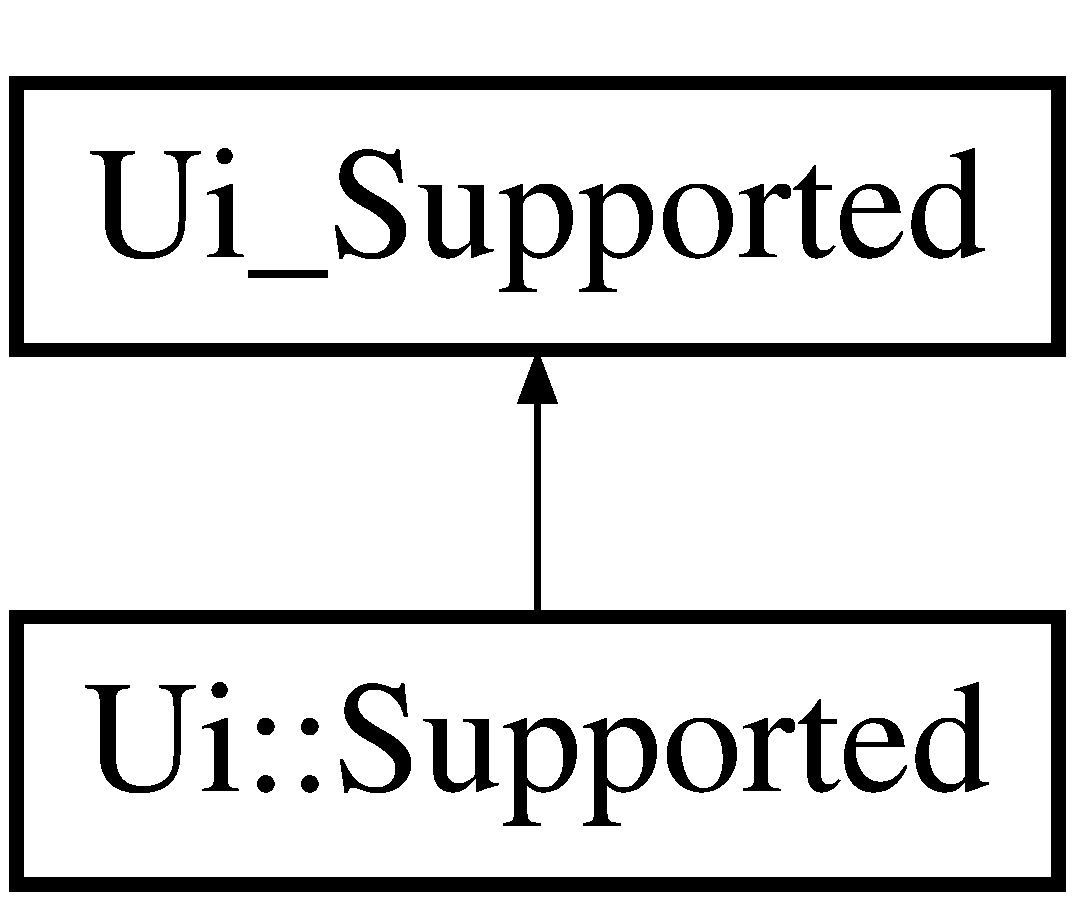
\includegraphics[height=2.000000cm]{classUi_1_1Supported}
\end{center}
\end{figure}
\subsection*{Additional Inherited Members}


The documentation for this class was generated from the following file\-:\begin{DoxyCompactItemize}
\item 
ui\-\_\-supported.\-h\end{DoxyCompactItemize}

\hypertarget{classSupported}{\section{Supported Class Reference}
\label{classSupported}\index{Supported@{Supported}}
}
Inheritance diagram for Supported\-:\begin{figure}[H]
\begin{center}
\leavevmode
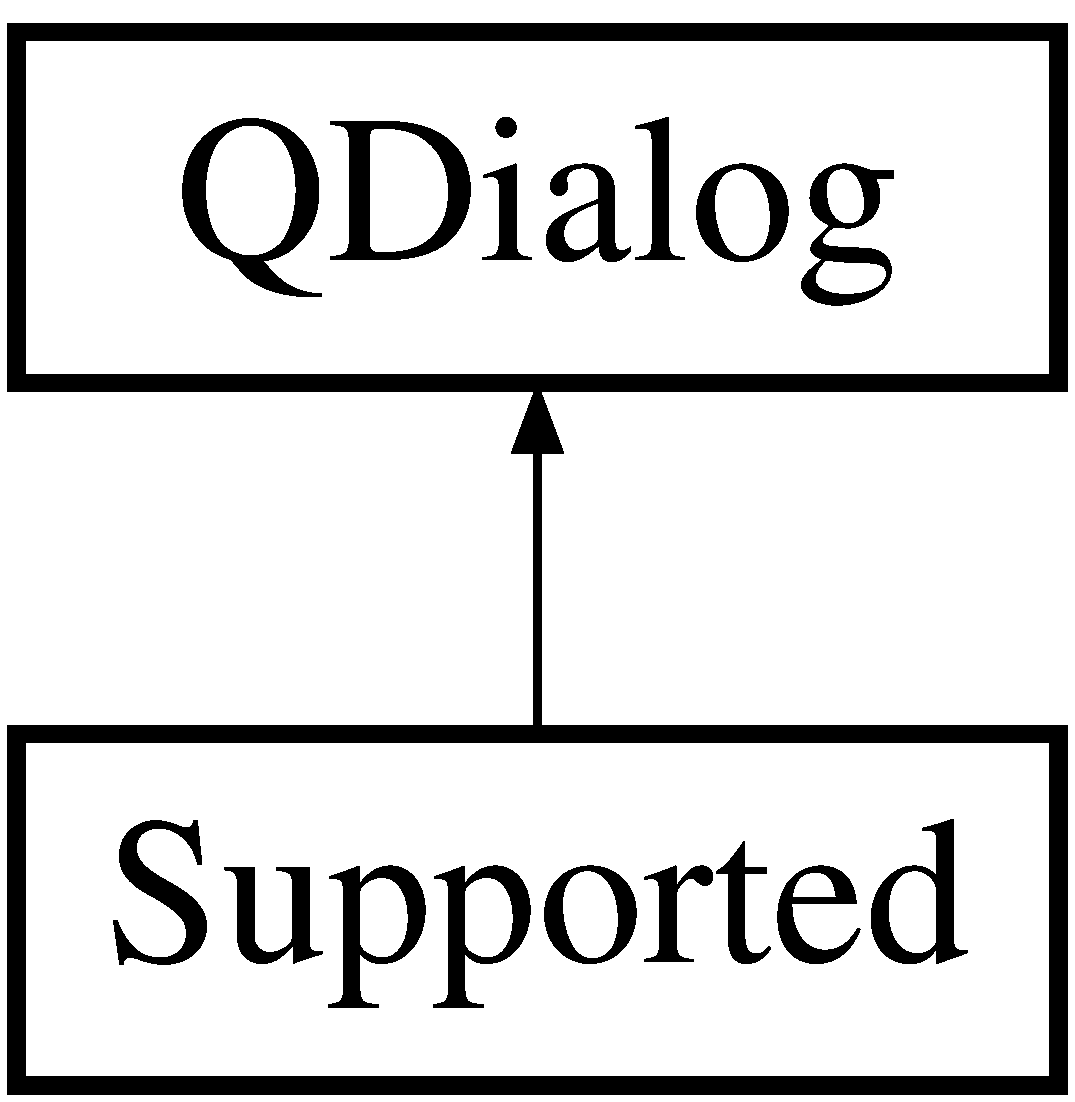
\includegraphics[height=2.000000cm]{classSupported}
\end{center}
\end{figure}
\subsection*{Public Member Functions}
\begin{DoxyCompactItemize}
\item 
\hypertarget{classSupported_a25d50afe2d3e394d407729dc58b0bc7d}{{\bfseries Supported} (Q\-Widget $\ast$parent=0)}\label{classSupported_a25d50afe2d3e394d407729dc58b0bc7d}

\end{DoxyCompactItemize}


The documentation for this class was generated from the following files\-:\begin{DoxyCompactItemize}
\item 
supported.\-h\item 
supported.\-cpp\end{DoxyCompactItemize}

\hypertarget{classTest__1}{\section{Test\-\_\-1 Class Reference}
\label{classTest__1}\index{Test\-\_\-1@{Test\-\_\-1}}
}
Inheritance diagram for Test\-\_\-1\-:\begin{figure}[H]
\begin{center}
\leavevmode
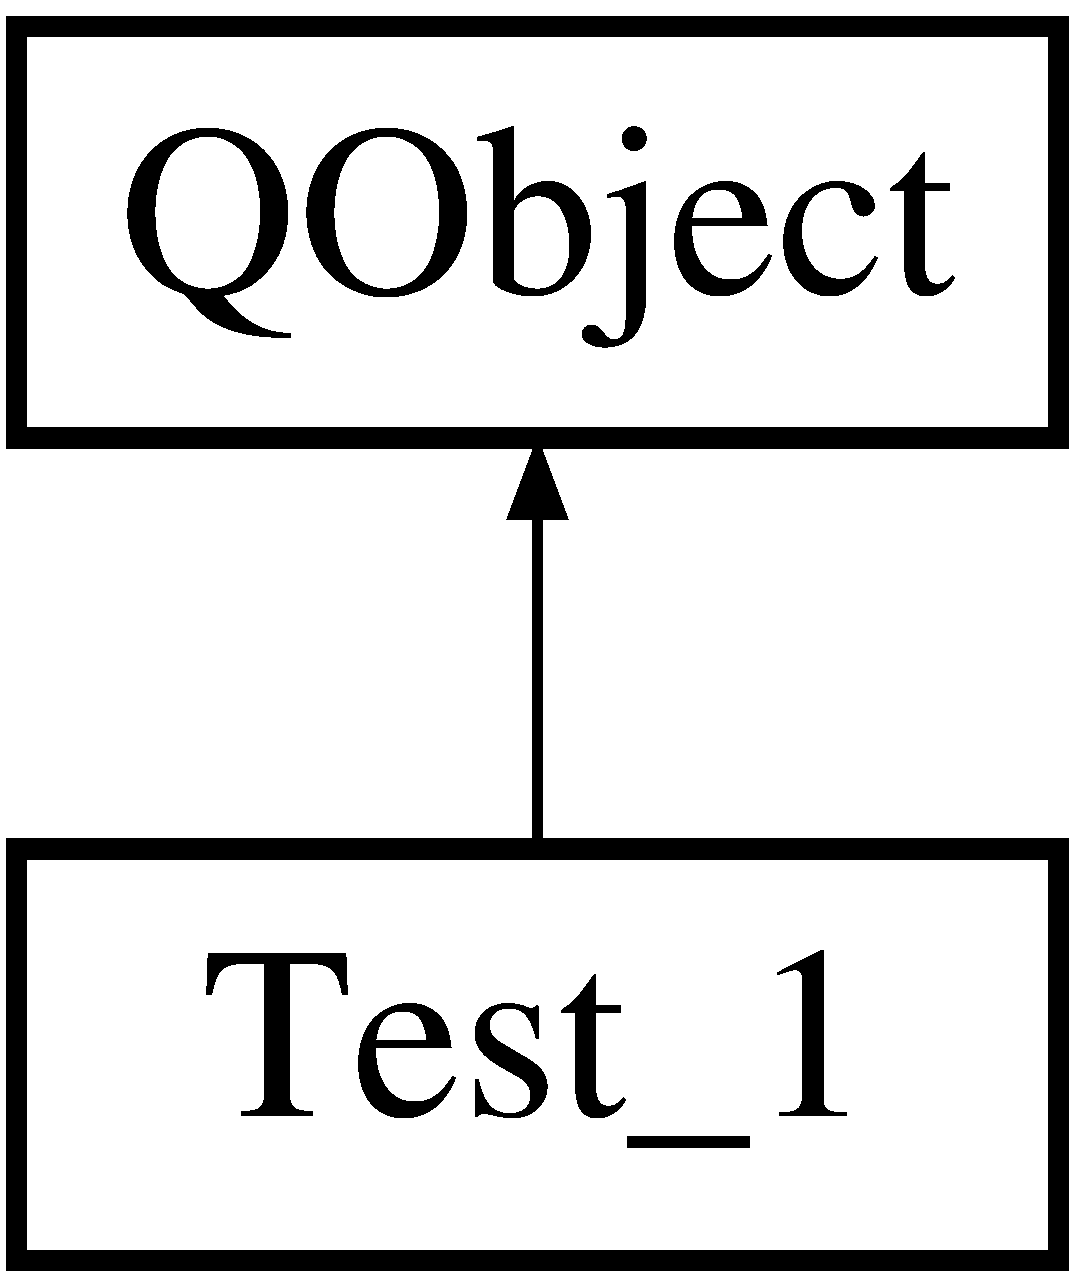
\includegraphics[height=2.000000cm]{classTest__1}
\end{center}
\end{figure}


The documentation for this class was generated from the following files\-:\begin{DoxyCompactItemize}
\item 
utests.\-h\item 
utests.\-cpp\end{DoxyCompactItemize}

\hypertarget{classUi__About}{\section{Ui\-\_\-\-About Class Reference}
\label{classUi__About}\index{Ui\-\_\-\-About@{Ui\-\_\-\-About}}
}
Inheritance diagram for Ui\-\_\-\-About\-:\begin{figure}[H]
\begin{center}
\leavevmode
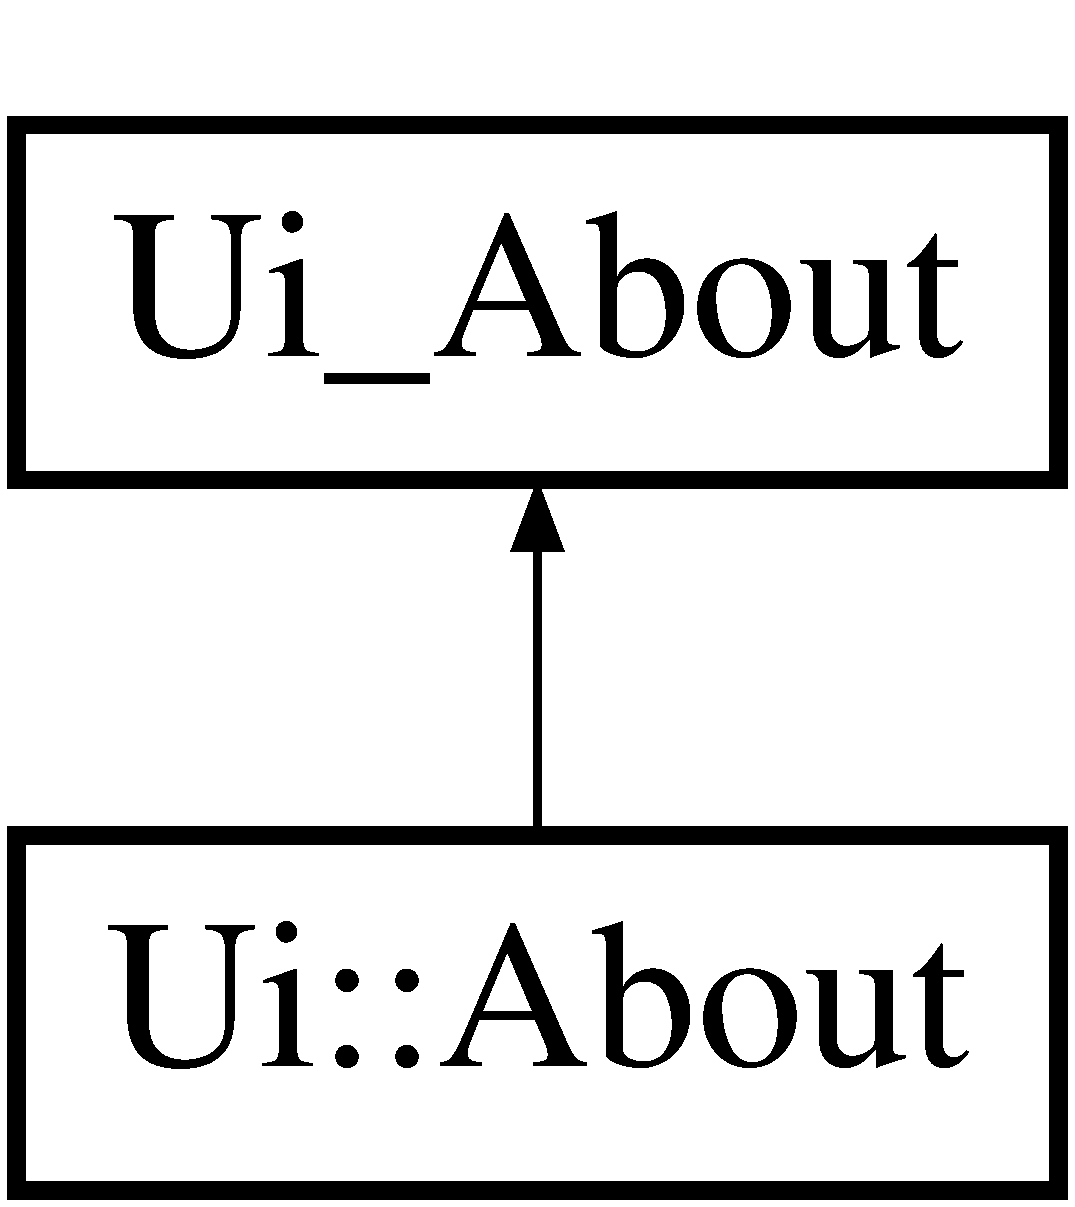
\includegraphics[height=2.000000cm]{classUi__About}
\end{center}
\end{figure}
\subsection*{Public Member Functions}
\begin{DoxyCompactItemize}
\item 
\hypertarget{classUi__About_a3f702c543d46b79f0d687e8a7711ebcb}{void {\bfseries setup\-Ui} (Q\-Dialog $\ast$\hyperlink{classAbout}{About})}\label{classUi__About_a3f702c543d46b79f0d687e8a7711ebcb}

\item 
\hypertarget{classUi__About_a6b1d5029f1ef8200024e6bf6b4fcebfc}{void {\bfseries retranslate\-Ui} (Q\-Dialog $\ast$\hyperlink{classAbout}{About})}\label{classUi__About_a6b1d5029f1ef8200024e6bf6b4fcebfc}

\end{DoxyCompactItemize}
\subsection*{Public Attributes}
\begin{DoxyCompactItemize}
\item 
\hypertarget{classUi__About_a785a67615301b1e09088e6b3b7becb2c}{Q\-Label $\ast$ {\bfseries l\-\_\-coreboot}}\label{classUi__About_a785a67615301b1e09088e6b3b7becb2c}

\item 
\hypertarget{classUi__About_adb3ba739fbbba64ea5da44ab36ed93a4}{Q\-Label $\ast$ {\bfseries l\-\_\-flashrom}}\label{classUi__About_adb3ba739fbbba64ea5da44ab36ed93a4}

\item 
\hypertarget{classUi__About_a46e929541dfcfcdae02585dd383fad53}{Q\-Label $\ast$ {\bfseries l\-\_\-coreboot\-\_\-ver}}\label{classUi__About_a46e929541dfcfcdae02585dd383fad53}

\item 
\hypertarget{classUi__About_acda4030ceb0520d40f60573e74fcf346}{Q\-Label $\ast$ {\bfseries l\-\_\-flashrom\-\_\-ver}}\label{classUi__About_acda4030ceb0520d40f60573e74fcf346}

\item 
\hypertarget{classUi__About_ab10fb3449495d26cdb07b48ee1b921f9}{Q\-Push\-Button $\ast$ {\bfseries b\-\_\-about\-\_\-close}}\label{classUi__About_ab10fb3449495d26cdb07b48ee1b921f9}

\end{DoxyCompactItemize}


The documentation for this class was generated from the following file\-:\begin{DoxyCompactItemize}
\item 
ui\-\_\-about.\-h\end{DoxyCompactItemize}

\hypertarget{classUi__AddComponent}{\section{Ui\-\_\-\-Add\-Component Class Reference}
\label{classUi__AddComponent}\index{Ui\-\_\-\-Add\-Component@{Ui\-\_\-\-Add\-Component}}
}
Inheritance diagram for Ui\-\_\-\-Add\-Component\-:\begin{figure}[H]
\begin{center}
\leavevmode
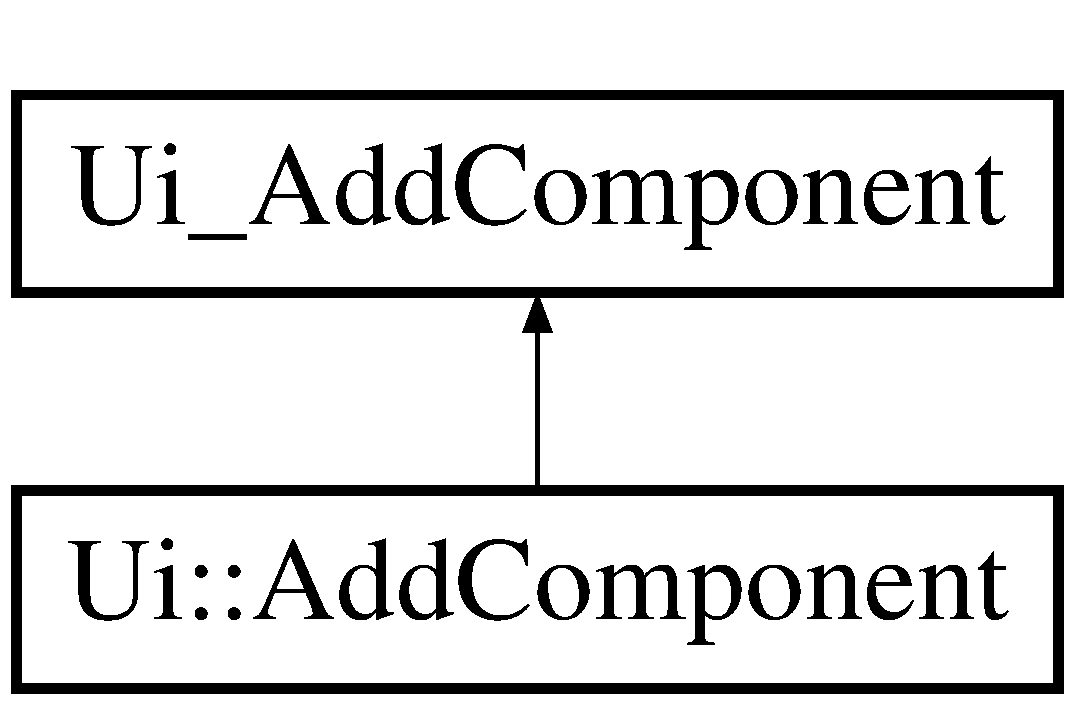
\includegraphics[height=2.000000cm]{classUi__AddComponent}
\end{center}
\end{figure}
\subsection*{Public Member Functions}
\begin{DoxyCompactItemize}
\item 
\hypertarget{classUi__AddComponent_acf348ed66a9a67dcc458ee2cbd809028}{void {\bfseries setup\-Ui} (Q\-Dialog $\ast$\hyperlink{classAddComponent}{Add\-Component})}\label{classUi__AddComponent_acf348ed66a9a67dcc458ee2cbd809028}

\item 
\hypertarget{classUi__AddComponent_a90f2c20d4af541e7d5f847df2edde6da}{void {\bfseries retranslate\-Ui} (Q\-Dialog $\ast$\hyperlink{classAddComponent}{Add\-Component})}\label{classUi__AddComponent_a90f2c20d4af541e7d5f847df2edde6da}

\end{DoxyCompactItemize}
\subsection*{Public Attributes}
\begin{DoxyCompactItemize}
\item 
\hypertarget{classUi__AddComponent_a3cec23b1fba8f525d03c48a22448189a}{Q\-Label $\ast$ {\bfseries l\-\_\-component}}\label{classUi__AddComponent_a3cec23b1fba8f525d03c48a22448189a}

\item 
\hypertarget{classUi__AddComponent_acbec0d71905737fab6c80a9e56f0414b}{Q\-Label $\ast$ {\bfseries l\-\_\-name}}\label{classUi__AddComponent_acbec0d71905737fab6c80a9e56f0414b}

\item 
\hypertarget{classUi__AddComponent_aa0038af0f41796d9978d32b77bda5008}{Q\-Line\-Edit $\ast$ {\bfseries edit\-\_\-name}}\label{classUi__AddComponent_aa0038af0f41796d9978d32b77bda5008}

\item 
\hypertarget{classUi__AddComponent_a563ee038186eda630b1c450481573a5b}{Q\-Push\-Button $\ast$ {\bfseries b\-\_\-add\-\_\-component}}\label{classUi__AddComponent_a563ee038186eda630b1c450481573a5b}

\item 
\hypertarget{classUi__AddComponent_ae9ff754bad272c80ceb80fce907bdddc}{Q\-Label $\ast$ {\bfseries l\-\_\-component\-\_\-name}}\label{classUi__AddComponent_ae9ff754bad272c80ceb80fce907bdddc}

\item 
\hypertarget{classUi__AddComponent_a57e17717b4eab4e2158171b50a17be12}{Q\-Push\-Button $\ast$ {\bfseries b\-\_\-sel\-\_\-component}}\label{classUi__AddComponent_a57e17717b4eab4e2158171b50a17be12}

\item 
\hypertarget{classUi__AddComponent_a6b03c43980b6ffdc8cd638a63c13ee66}{Q\-Label $\ast$ {\bfseries l\-\_\-type}}\label{classUi__AddComponent_a6b03c43980b6ffdc8cd638a63c13ee66}

\item 
\hypertarget{classUi__AddComponent_a3407ea1f66fdff7d2d5ad7f1e111b2c3}{Q\-Combo\-Box $\ast$ {\bfseries cb\-\_\-sel\-\_\-type}}\label{classUi__AddComponent_a3407ea1f66fdff7d2d5ad7f1e111b2c3}

\end{DoxyCompactItemize}


The documentation for this class was generated from the following file\-:\begin{DoxyCompactItemize}
\item 
ui\-\_\-addcomponent.\-h\end{DoxyCompactItemize}

\hypertarget{classUi__ChooseChip}{\section{Ui\-\_\-\-Choose\-Chip Class Reference}
\label{classUi__ChooseChip}\index{Ui\-\_\-\-Choose\-Chip@{Ui\-\_\-\-Choose\-Chip}}
}
Inheritance diagram for Ui\-\_\-\-Choose\-Chip\-:\begin{figure}[H]
\begin{center}
\leavevmode
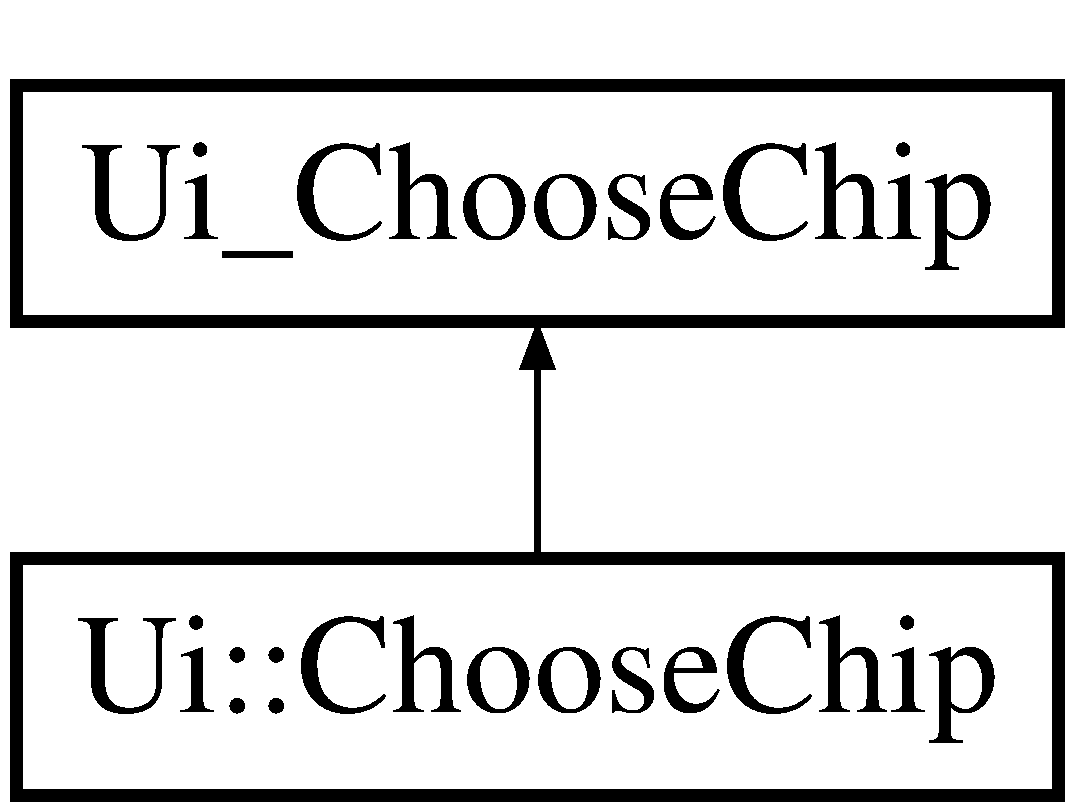
\includegraphics[height=2.000000cm]{classUi__ChooseChip}
\end{center}
\end{figure}
\subsection*{Public Member Functions}
\begin{DoxyCompactItemize}
\item 
\hypertarget{classUi__ChooseChip_a8b1b7532ad7acf8776500245b9ced193}{void {\bfseries setup\-Ui} (Q\-Dialog $\ast$\hyperlink{classChooseChip}{Choose\-Chip})}\label{classUi__ChooseChip_a8b1b7532ad7acf8776500245b9ced193}

\item 
\hypertarget{classUi__ChooseChip_a458d4ba1d1ed78eb156a08d030061841}{void {\bfseries retranslate\-Ui} (Q\-Dialog $\ast$\hyperlink{classChooseChip}{Choose\-Chip})}\label{classUi__ChooseChip_a458d4ba1d1ed78eb156a08d030061841}

\end{DoxyCompactItemize}
\subsection*{Public Attributes}
\begin{DoxyCompactItemize}
\item 
\hypertarget{classUi__ChooseChip_a855422798025d2b9f9c61d20cc243c33}{Q\-List\-Widget $\ast$ {\bfseries chip\-\_\-list}}\label{classUi__ChooseChip_a855422798025d2b9f9c61d20cc243c33}

\item 
\hypertarget{classUi__ChooseChip_a271aa8a7a94ba1d6e0e45a4c8b0dcdbd}{Q\-Push\-Button $\ast$ {\bfseries b\-\_\-chip\-\_\-ok}}\label{classUi__ChooseChip_a271aa8a7a94ba1d6e0e45a4c8b0dcdbd}

\end{DoxyCompactItemize}


The documentation for this class was generated from the following file\-:\begin{DoxyCompactItemize}
\item 
ui\-\_\-choosechip.\-h\end{DoxyCompactItemize}

\hypertarget{classUi__DeleteComponents}{\section{Ui\-\_\-\-Delete\-Components Class Reference}
\label{classUi__DeleteComponents}\index{Ui\-\_\-\-Delete\-Components@{Ui\-\_\-\-Delete\-Components}}
}
Inheritance diagram for Ui\-\_\-\-Delete\-Components\-:\begin{figure}[H]
\begin{center}
\leavevmode
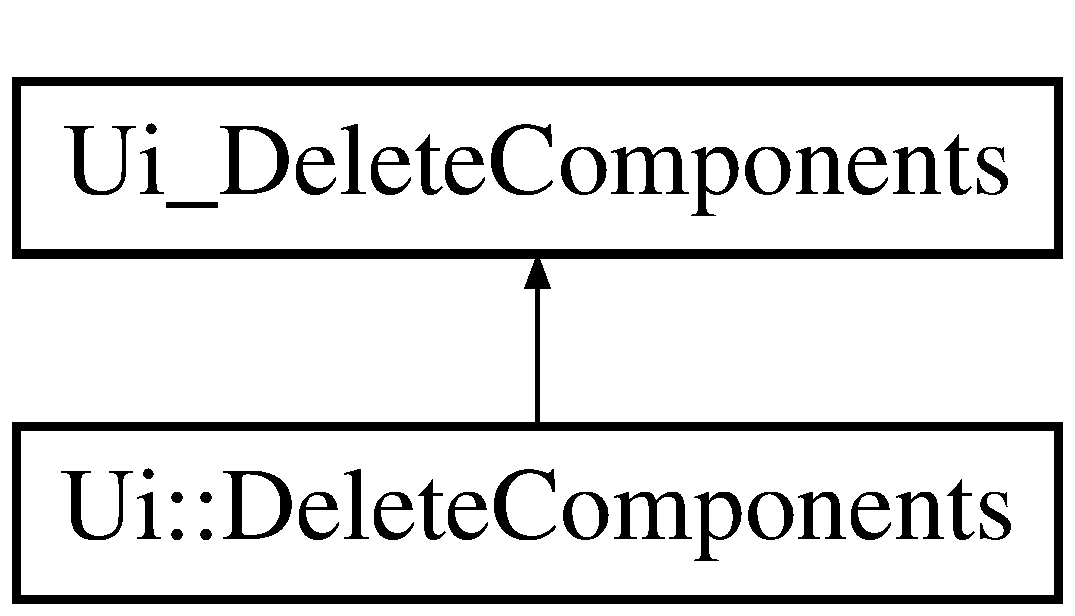
\includegraphics[height=2.000000cm]{classUi__DeleteComponents}
\end{center}
\end{figure}
\subsection*{Public Member Functions}
\begin{DoxyCompactItemize}
\item 
\hypertarget{classUi__DeleteComponents_a3d20b977ef8f335cd8b0ec2b2ab89453}{void {\bfseries setup\-Ui} (Q\-Dialog $\ast$\hyperlink{classDeleteComponents}{Delete\-Components})}\label{classUi__DeleteComponents_a3d20b977ef8f335cd8b0ec2b2ab89453}

\item 
\hypertarget{classUi__DeleteComponents_a4b5bfca255829b23527e483457ba47d1}{void {\bfseries retranslate\-Ui} (Q\-Dialog $\ast$\hyperlink{classDeleteComponents}{Delete\-Components})}\label{classUi__DeleteComponents_a4b5bfca255829b23527e483457ba47d1}

\end{DoxyCompactItemize}
\subsection*{Public Attributes}
\begin{DoxyCompactItemize}
\item 
\hypertarget{classUi__DeleteComponents_a741526d789f0a5485fcafc2bb6881d42}{Q\-Line\-Edit $\ast$ {\bfseries edit\-\_\-name}}\label{classUi__DeleteComponents_a741526d789f0a5485fcafc2bb6881d42}

\item 
\hypertarget{classUi__DeleteComponents_a99b79751b6675c91f8ad8f26741dc4cb}{Q\-Label $\ast$ {\bfseries l\-\_\-name}}\label{classUi__DeleteComponents_a99b79751b6675c91f8ad8f26741dc4cb}

\item 
\hypertarget{classUi__DeleteComponents_ac6a29156a3a81464f2539e61e65004ce}{Q\-Push\-Button $\ast$ {\bfseries b\-\_\-remove\-\_\-comp}}\label{classUi__DeleteComponents_ac6a29156a3a81464f2539e61e65004ce}

\end{DoxyCompactItemize}


The documentation for this class was generated from the following file\-:\begin{DoxyCompactItemize}
\item 
ui\-\_\-deletecomponents.\-h\end{DoxyCompactItemize}

\hypertarget{classUi__InfoDialog}{\section{Ui\-\_\-\-Info\-Dialog Class Reference}
\label{classUi__InfoDialog}\index{Ui\-\_\-\-Info\-Dialog@{Ui\-\_\-\-Info\-Dialog}}
}
Inheritance diagram for Ui\-\_\-\-Info\-Dialog\-:\begin{figure}[H]
\begin{center}
\leavevmode
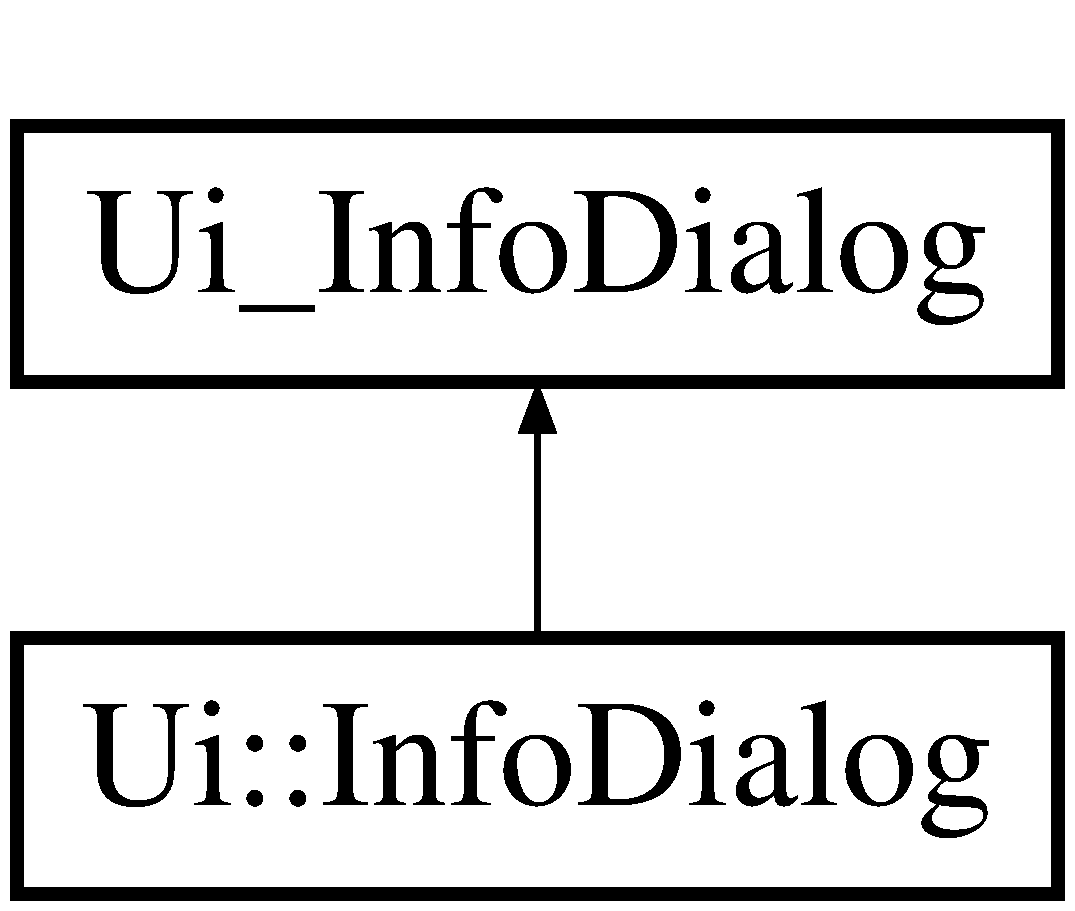
\includegraphics[height=2.000000cm]{classUi__InfoDialog}
\end{center}
\end{figure}
\subsection*{Public Member Functions}
\begin{DoxyCompactItemize}
\item 
\hypertarget{classUi__InfoDialog_a86ee02737f691e3537404a42e79cf19a}{void {\bfseries setup\-Ui} (Q\-Dialog $\ast$\hyperlink{classInfoDialog}{Info\-Dialog})}\label{classUi__InfoDialog_a86ee02737f691e3537404a42e79cf19a}

\item 
\hypertarget{classUi__InfoDialog_a017e4da9fab727a21f7ba83bb689d434}{void {\bfseries retranslate\-Ui} (Q\-Dialog $\ast$\hyperlink{classInfoDialog}{Info\-Dialog})}\label{classUi__InfoDialog_a017e4da9fab727a21f7ba83bb689d434}

\end{DoxyCompactItemize}
\subsection*{Public Attributes}
\begin{DoxyCompactItemize}
\item 
\hypertarget{classUi__InfoDialog_af7e4d2cf7d5cd3f1525b683485a1ec63}{Q\-Label $\ast$ {\bfseries l\-\_\-info}}\label{classUi__InfoDialog_af7e4d2cf7d5cd3f1525b683485a1ec63}

\item 
\hypertarget{classUi__InfoDialog_a7b16d0aaa4f153f43e6df491d8d5f9f3}{Q\-Push\-Button $\ast$ {\bfseries b\-\_\-ok}}\label{classUi__InfoDialog_a7b16d0aaa4f153f43e6df491d8d5f9f3}

\end{DoxyCompactItemize}


The documentation for this class was generated from the following file\-:\begin{DoxyCompactItemize}
\item 
ui\-\_\-infodialog.\-h\end{DoxyCompactItemize}

\hypertarget{classUi__MainWindow}{\section{Ui\-\_\-\-Main\-Window Class Reference}
\label{classUi__MainWindow}\index{Ui\-\_\-\-Main\-Window@{Ui\-\_\-\-Main\-Window}}
}
Inheritance diagram for Ui\-\_\-\-Main\-Window\-:\begin{figure}[H]
\begin{center}
\leavevmode
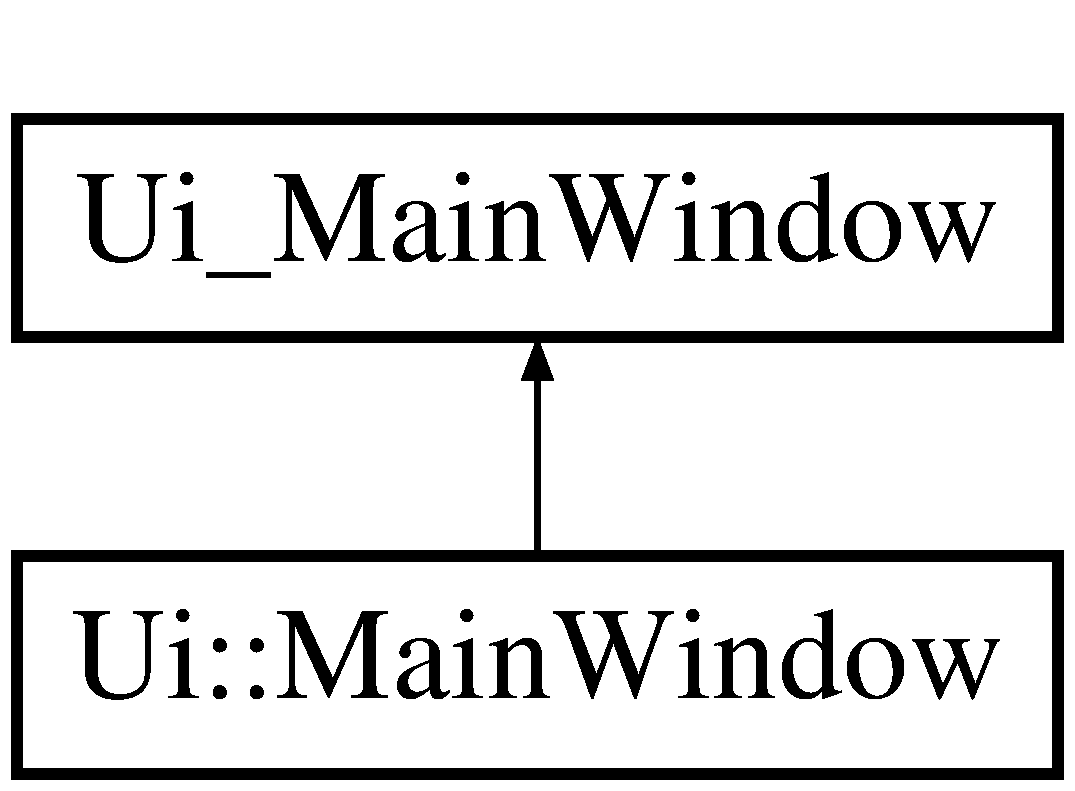
\includegraphics[height=2.000000cm]{classUi__MainWindow}
\end{center}
\end{figure}
\subsection*{Public Member Functions}
\begin{DoxyCompactItemize}
\item 
\hypertarget{classUi__MainWindow_acf4a0872c4c77d8f43a2ec66ed849b58}{void {\bfseries setup\-Ui} (Q\-Main\-Window $\ast$\hyperlink{classMainWindow}{Main\-Window})}\label{classUi__MainWindow_acf4a0872c4c77d8f43a2ec66ed849b58}

\item 
\hypertarget{classUi__MainWindow_a097dd160c3534a204904cb374412c618}{void {\bfseries retranslate\-Ui} (Q\-Main\-Window $\ast$\hyperlink{classMainWindow}{Main\-Window})}\label{classUi__MainWindow_a097dd160c3534a204904cb374412c618}

\end{DoxyCompactItemize}
\subsection*{Public Attributes}
\begin{DoxyCompactItemize}
\item 
\hypertarget{classUi__MainWindow_aab4b28ba129cf41b95caced7769f1069}{Q\-Action $\ast$ {\bfseries act\-\_\-about}}\label{classUi__MainWindow_aab4b28ba129cf41b95caced7769f1069}

\item 
\hypertarget{classUi__MainWindow_a907125233437d6db0cc0473193058912}{Q\-Action $\ast$ {\bfseries act\-\_\-supported\-\_\-list}}\label{classUi__MainWindow_a907125233437d6db0cc0473193058912}

\item 
\hypertarget{classUi__MainWindow_ae77f9aab6b3f14a8c32153888e45cc7d}{Q\-Action $\ast$ {\bfseries act\-\_\-preferences}}\label{classUi__MainWindow_ae77f9aab6b3f14a8c32153888e45cc7d}

\item 
\hypertarget{classUi__MainWindow_a30075506c2116c3ed4ff25e07ae75f81}{Q\-Widget $\ast$ {\bfseries central\-Widget}}\label{classUi__MainWindow_a30075506c2116c3ed4ff25e07ae75f81}

\item 
\hypertarget{classUi__MainWindow_aaca249d901914381e98dd2b7910086ab}{Q\-Label $\ast$ {\bfseries l\-\_\-prog\-\_\-name}}\label{classUi__MainWindow_aaca249d901914381e98dd2b7910086ab}

\item 
\hypertarget{classUi__MainWindow_a3260b943854b841c986f47c4726ee7f9}{Q\-Tab\-Widget $\ast$ {\bfseries tab\-Widget}}\label{classUi__MainWindow_a3260b943854b841c986f47c4726ee7f9}

\item 
\hypertarget{classUi__MainWindow_a9262538a700c6a9c0ead582913a05540}{Q\-Widget $\ast$ {\bfseries tab\-\_\-auto}}\label{classUi__MainWindow_a9262538a700c6a9c0ead582913a05540}

\item 
\hypertarget{classUi__MainWindow_a51ae27370c9f75439dc9b9e89983c3de}{Q\-Label $\ast$ {\bfseries l\-\_\-auto\-\_\-payload}}\label{classUi__MainWindow_a51ae27370c9f75439dc9b9e89983c3de}

\item 
\hypertarget{classUi__MainWindow_a620f01689f782082eac85ca17ead4ce4}{Q\-Combo\-Box $\ast$ {\bfseries cb\-\_\-auto\-\_\-sel\-\_\-payload}}\label{classUi__MainWindow_a620f01689f782082eac85ca17ead4ce4}

\item 
\hypertarget{classUi__MainWindow_ad4a3ea0c03415c5f9b38bbe4e9cf8f61}{Q\-Text\-Edit $\ast$ {\bfseries log\-\_\-auto}}\label{classUi__MainWindow_ad4a3ea0c03415c5f9b38bbe4e9cf8f61}

\item 
\hypertarget{classUi__MainWindow_acd8db516196c88222683824da3dc9919}{Q\-Push\-Button $\ast$ {\bfseries b\-\_\-auto\-\_\-flash}}\label{classUi__MainWindow_acd8db516196c88222683824da3dc9919}

\item 
\hypertarget{classUi__MainWindow_ab4c28a77764fac053804b3b2efb3c3af}{Q\-Push\-Button $\ast$ {\bfseries b\-\_\-auto\-\_\-get\-\_\-hw\-\_\-data}}\label{classUi__MainWindow_ab4c28a77764fac053804b3b2efb3c3af}

\item 
\hypertarget{classUi__MainWindow_acb63584eb149725252772bc7be693ab0}{Q\-Push\-Button $\ast$ {\bfseries b\-\_\-auto\-\_\-build\-\_\-img}}\label{classUi__MainWindow_acb63584eb149725252772bc7be693ab0}

\item 
\hypertarget{classUi__MainWindow_a8722b474130b0ca7d039d201365c5015}{Q\-Push\-Button $\ast$ {\bfseries b\-\_\-auto\-\_\-get\-\_\-bios}}\label{classUi__MainWindow_a8722b474130b0ca7d039d201365c5015}

\item 
\hypertarget{classUi__MainWindow_a69258f781d1d148c486cf4e0287700cf}{Q\-Push\-Button $\ast$ {\bfseries b\-\_\-auto\-\_\-set\-\_\-bios}}\label{classUi__MainWindow_a69258f781d1d148c486cf4e0287700cf}

\item 
\hypertarget{classUi__MainWindow_a07e6f7d1c8cc34539aa60b138b2a82f3}{Q\-Widget $\ast$ {\bfseries tab\-\_\-flash}}\label{classUi__MainWindow_a07e6f7d1c8cc34539aa60b138b2a82f3}

\item 
\hypertarget{classUi__MainWindow_ae89606905cfa404ce84a511345e20599}{Q\-Push\-Button $\ast$ {\bfseries b\-\_\-read}}\label{classUi__MainWindow_ae89606905cfa404ce84a511345e20599}

\item 
\hypertarget{classUi__MainWindow_a5825182d63b281d5acc32c6efacff6ae}{Q\-Push\-Button $\ast$ {\bfseries b\-\_\-erase}}\label{classUi__MainWindow_a5825182d63b281d5acc32c6efacff6ae}

\item 
\hypertarget{classUi__MainWindow_abb4e3ee3b5b7c9ce312276582e9b30fd}{Q\-Push\-Button $\ast$ {\bfseries b\-\_\-flash}}\label{classUi__MainWindow_abb4e3ee3b5b7c9ce312276582e9b30fd}

\item 
\hypertarget{classUi__MainWindow_ad67401f8f0e2b76cb648e3ad396efa3c}{Q\-Text\-Edit $\ast$ {\bfseries log\-\_\-flash}}\label{classUi__MainWindow_ad67401f8f0e2b76cb648e3ad396efa3c}

\item 
\hypertarget{classUi__MainWindow_affd9d88440a5b7c050264aafe32d62ff}{Q\-Push\-Button $\ast$ {\bfseries b\-\_\-verify}}\label{classUi__MainWindow_affd9d88440a5b7c050264aafe32d62ff}

\item 
\hypertarget{classUi__MainWindow_afb6c29200ea885957744bbd71c9ef636}{Q\-Push\-Button $\ast$ {\bfseries b\-\_\-probe}}\label{classUi__MainWindow_afb6c29200ea885957744bbd71c9ef636}

\item 
\hypertarget{classUi__MainWindow_a81200101d4f9a357cf3fe3fa5bc5aa0d}{Q\-Widget $\ast$ {\bfseries tab\-\_\-rom\-\_\-options}}\label{classUi__MainWindow_a81200101d4f9a357cf3fe3fa5bc5aa0d}

\item 
\hypertarget{classUi__MainWindow_ab66e727d962165698210fcb733bf8dc4}{Q\-Push\-Button $\ast$ {\bfseries b\-\_\-remove\-\_\-comp}}\label{classUi__MainWindow_ab66e727d962165698210fcb733bf8dc4}

\item 
\hypertarget{classUi__MainWindow_a71b52f98997a76659cc6a791923a9c6f}{Q\-Label $\ast$ {\bfseries l\-\_\-opt\-\_\-rom}}\label{classUi__MainWindow_a71b52f98997a76659cc6a791923a9c6f}

\item 
\hypertarget{classUi__MainWindow_a1b65a6887c743491285911992d20dc6f}{Q\-Push\-Button $\ast$ {\bfseries b\-\_\-add\-\_\-component}}\label{classUi__MainWindow_a1b65a6887c743491285911992d20dc6f}

\item 
\hypertarget{classUi__MainWindow_a30ba28fca193c5bb8444b0f25abad69b}{Q\-Table\-View $\ast$ {\bfseries tv\-\_\-rom\-\_\-content}}\label{classUi__MainWindow_a30ba28fca193c5bb8444b0f25abad69b}

\item 
\hypertarget{classUi__MainWindow_ae2f2b2a9da0f259dc8576280c5eac744}{Q\-Text\-Edit $\ast$ {\bfseries log\-\_\-rom\-\_\-opt}}\label{classUi__MainWindow_ae2f2b2a9da0f259dc8576280c5eac744}

\item 
\hypertarget{classUi__MainWindow_a70d438b5ad5fae5ff8b4f18842a6bbfc}{Q\-Push\-Button $\ast$ {\bfseries b\-\_\-ropt\-\_\-select}}\label{classUi__MainWindow_a70d438b5ad5fae5ff8b4f18842a6bbfc}

\item 
\hypertarget{classUi__MainWindow_a8032f9a0895de06a08c227dbc93f9d04}{Q\-Widget $\ast$ {\bfseries tab\-\_\-extract}}\label{classUi__MainWindow_a8032f9a0895de06a08c227dbc93f9d04}

\item 
\hypertarget{classUi__MainWindow_a3e0210034aba9c6ee9a9a3538e31cef9}{Q\-Label $\ast$ {\bfseries l\-\_\-ex\-\_\-rom}}\label{classUi__MainWindow_a3e0210034aba9c6ee9a9a3538e31cef9}

\item 
\hypertarget{classUi__MainWindow_a0d5394b7fa01c1666f6d10d639fcc385}{Q\-Label $\ast$ {\bfseries l\-\_\-ex\-\_\-output}}\label{classUi__MainWindow_a0d5394b7fa01c1666f6d10d639fcc385}

\item 
\hypertarget{classUi__MainWindow_a6b58128efccb33a4e76650a8cad7b66e}{Q\-Label $\ast$ {\bfseries l\-\_\-ex\-\_\-rom\-\_\-name}}\label{classUi__MainWindow_a6b58128efccb33a4e76650a8cad7b66e}

\item 
\hypertarget{classUi__MainWindow_aa1c846f04d30b9c57cb1a8f6708e38bd}{Q\-Push\-Button $\ast$ {\bfseries b\-\_\-sel\-\_\-bios\-\_\-rom}}\label{classUi__MainWindow_aa1c846f04d30b9c57cb1a8f6708e38bd}

\item 
\hypertarget{classUi__MainWindow_a225860466a4cfbd53c2a40fd41230f39}{Q\-Push\-Button $\ast$ {\bfseries b\-\_\-extract}}\label{classUi__MainWindow_a225860466a4cfbd53c2a40fd41230f39}

\item 
\hypertarget{classUi__MainWindow_aaf6ee8afd383315d2c1d9439359459a9}{Q\-Text\-Edit $\ast$ {\bfseries log\-\_\-extract}}\label{classUi__MainWindow_aaf6ee8afd383315d2c1d9439359459a9}

\item 
\hypertarget{classUi__MainWindow_abe4cf601281bad2b9725366c76f72cc3}{Q\-Label $\ast$ {\bfseries l\-\_\-ex\-\_\-out\-\_\-name}}\label{classUi__MainWindow_abe4cf601281bad2b9725366c76f72cc3}

\item 
\hypertarget{classUi__MainWindow_a99eb1f5c8c287e6a1d69272ea0124615}{Q\-Push\-Button $\ast$ {\bfseries b\-\_\-sel\-\_\-bios\-\_\-out}}\label{classUi__MainWindow_a99eb1f5c8c287e6a1d69272ea0124615}

\item 
\hypertarget{classUi__MainWindow_a3eefc97e77c01b693c6c250045b04752}{Q\-Widget $\ast$ {\bfseries tab\-\_\-create\-\_\-rom}}\label{classUi__MainWindow_a3eefc97e77c01b693c6c250045b04752}

\item 
\hypertarget{classUi__MainWindow_a09300c87f9c25e765dbad68fa8e6168b}{Q\-Label $\ast$ {\bfseries l\-\_\-architecture}}\label{classUi__MainWindow_a09300c87f9c25e765dbad68fa8e6168b}

\item 
\hypertarget{classUi__MainWindow_aca8d3589d06dafab00e83bbc7280ac5f}{Q\-Label $\ast$ {\bfseries l\-\_\-bb\-\_\-offset}}\label{classUi__MainWindow_aca8d3589d06dafab00e83bbc7280ac5f}

\item 
\hypertarget{classUi__MainWindow_a1b0392315b38fd4a3e490c389d45f7d5}{Q\-Label $\ast$ {\bfseries l\-\_\-cbfs\-\_\-offset}}\label{classUi__MainWindow_a1b0392315b38fd4a3e490c389d45f7d5}

\item 
\hypertarget{classUi__MainWindow_af3de0b78e844c626ce487c3de3e2184b}{Q\-Label $\ast$ {\bfseries l\-\_\-bootblock}}\label{classUi__MainWindow_af3de0b78e844c626ce487c3de3e2184b}

\item 
\hypertarget{classUi__MainWindow_abe072612da1198bb87a3ae8805b01882}{Q\-Line\-Edit $\ast$ {\bfseries edit\-\_\-bootblock\-\_\-off}}\label{classUi__MainWindow_abe072612da1198bb87a3ae8805b01882}

\item 
\hypertarget{classUi__MainWindow_a518d14802c75b2f855804c4ad060772c}{Q\-Line\-Edit $\ast$ {\bfseries edit\-\_\-cbfs\-\_\-off}}\label{classUi__MainWindow_a518d14802c75b2f855804c4ad060772c}

\item 
\hypertarget{classUi__MainWindow_ae199dcf94d2b6437f043722e208bf163}{Q\-Push\-Button $\ast$ {\bfseries b\-\_\-sel\-\_\-boot\-\_\-block}}\label{classUi__MainWindow_ae199dcf94d2b6437f043722e208bf163}

\item 
\hypertarget{classUi__MainWindow_a3691bf7adcb903b244cb4afc4bd3ed39}{Q\-Combo\-Box $\ast$ {\bfseries cb\-\_\-sel\-\_\-arch}}\label{classUi__MainWindow_a3691bf7adcb903b244cb4afc4bd3ed39}

\item 
\hypertarget{classUi__MainWindow_ade15aeca25e4efb76382fe29cb961d6d}{Q\-Push\-Button $\ast$ {\bfseries b\-\_\-create\-\_\-rom}}\label{classUi__MainWindow_ade15aeca25e4efb76382fe29cb961d6d}

\item 
\hypertarget{classUi__MainWindow_a87647a4403864528eca99cdbf35e548f}{Q\-Text\-Edit $\ast$ {\bfseries log\-\_\-create\-\_\-rom}}\label{classUi__MainWindow_a87647a4403864528eca99cdbf35e548f}

\item 
\hypertarget{classUi__MainWindow_a9789b3ba149fc48b9499f53717724919}{Q\-Label $\ast$ {\bfseries l\-\_\-bootblack\-\_\-name}}\label{classUi__MainWindow_a9789b3ba149fc48b9499f53717724919}

\item 
\hypertarget{classUi__MainWindow_a2e2516d755e4dd53fc905dabddf2738a}{Q\-Label $\ast$ {\bfseries label\-\_\-2}}\label{classUi__MainWindow_a2e2516d755e4dd53fc905dabddf2738a}

\item 
\hypertarget{classUi__MainWindow_ae70a8f0d7adf85d25a51a631ef9f0d0f}{Q\-Line\-Edit $\ast$ {\bfseries edit\-\_\-cbfs\-\_\-name}}\label{classUi__MainWindow_ae70a8f0d7adf85d25a51a631ef9f0d0f}

\item 
\hypertarget{classUi__MainWindow_a5ddb567c63c98403128579b8f1aecdf4}{Q\-Label $\ast$ {\bfseries l\-\_\-size}}\label{classUi__MainWindow_a5ddb567c63c98403128579b8f1aecdf4}

\item 
\hypertarget{classUi__MainWindow_aa6f4a6e95d8b144f900f2b5688bf39d9}{Q\-Line\-Edit $\ast$ {\bfseries edit\-\_\-size}}\label{classUi__MainWindow_aa6f4a6e95d8b144f900f2b5688bf39d9}

\item 
\hypertarget{classUi__MainWindow_aaa0bd5d6c810aaf66c7d5842d4e89508}{Q\-Combo\-Box $\ast$ {\bfseries cb\-\_\-sel\-\_\-progr}}\label{classUi__MainWindow_aaa0bd5d6c810aaf66c7d5842d4e89508}

\item 
\hypertarget{classUi__MainWindow_a92874f8d6577fbf029b2825492a4a9b3}{Q\-Label $\ast$ {\bfseries l\-\_\-programmer}}\label{classUi__MainWindow_a92874f8d6577fbf029b2825492a4a9b3}

\item 
\hypertarget{classUi__MainWindow_ae3ae3c73fdcc9027fa07800d29071b6e}{Q\-Label $\ast$ {\bfseries l\-\_\-prog\-\_\-param}}\label{classUi__MainWindow_ae3ae3c73fdcc9027fa07800d29071b6e}

\item 
\hypertarget{classUi__MainWindow_a2ca19c85487f3a52b494bbe1ff9838ab}{Q\-Line\-Edit $\ast$ {\bfseries edit\-\_\-prog\-\_\-param}}\label{classUi__MainWindow_a2ca19c85487f3a52b494bbe1ff9838ab}

\item 
\hypertarget{classUi__MainWindow_a4f25747d8bfe22d1a3abba88dddd5661}{Q\-Push\-Button $\ast$ {\bfseries b\-\_\-init\-\_\-prog}}\label{classUi__MainWindow_a4f25747d8bfe22d1a3abba88dddd5661}

\item 
\hypertarget{classUi__MainWindow_a5172877001c8c7b4e0f6de50421867d1}{Q\-Tool\-Bar $\ast$ {\bfseries main\-Tool\-Bar}}\label{classUi__MainWindow_a5172877001c8c7b4e0f6de50421867d1}

\item 
\hypertarget{classUi__MainWindow_a50fa481337604bcc8bf68de18ab16ecd}{Q\-Status\-Bar $\ast$ {\bfseries status\-Bar}}\label{classUi__MainWindow_a50fa481337604bcc8bf68de18ab16ecd}

\end{DoxyCompactItemize}


The documentation for this class was generated from the following file\-:\begin{DoxyCompactItemize}
\item 
ui\-\_\-mainwindow.\-h\end{DoxyCompactItemize}

\hypertarget{classUi__Preferences}{\section{Ui\-\_\-\-Preferences Class Reference}
\label{classUi__Preferences}\index{Ui\-\_\-\-Preferences@{Ui\-\_\-\-Preferences}}
}
Inheritance diagram for Ui\-\_\-\-Preferences\-:\begin{figure}[H]
\begin{center}
\leavevmode
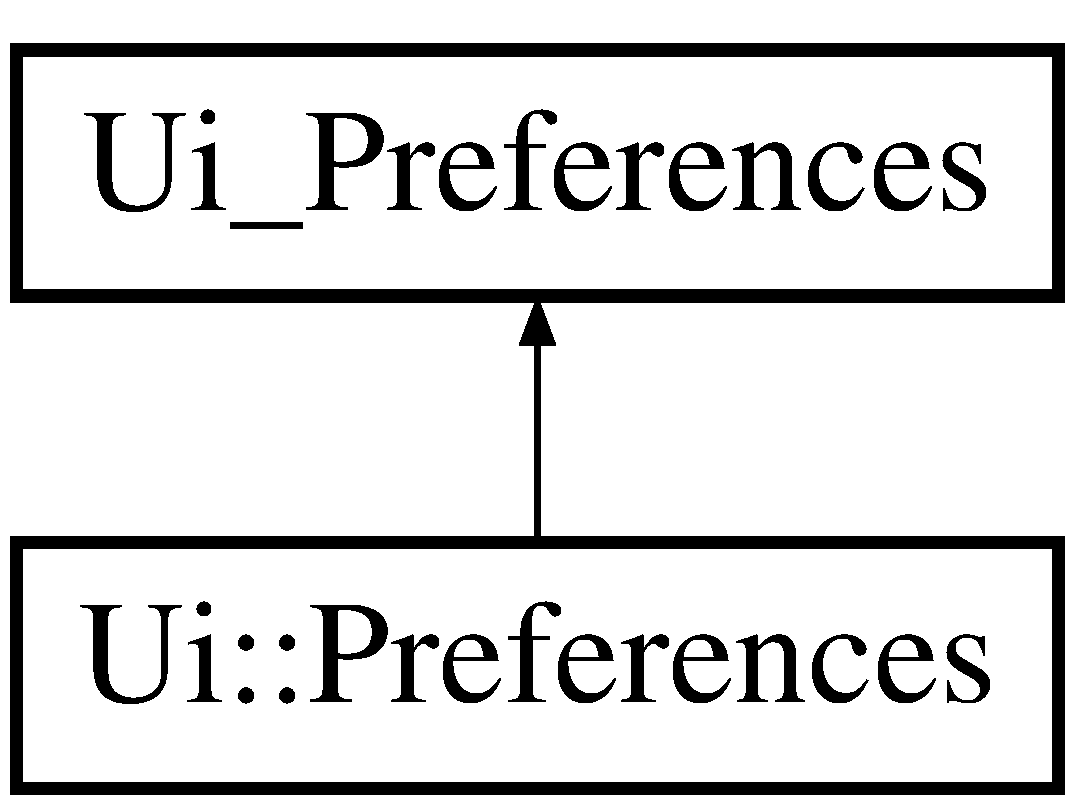
\includegraphics[height=2.000000cm]{classUi__Preferences}
\end{center}
\end{figure}
\subsection*{Public Member Functions}
\begin{DoxyCompactItemize}
\item 
\hypertarget{classUi__Preferences_a2c535ca36a3133132a7c858a4972df85}{void {\bfseries setup\-Ui} (Q\-Dialog $\ast$\hyperlink{classPreferences}{Preferences})}\label{classUi__Preferences_a2c535ca36a3133132a7c858a4972df85}

\item 
\hypertarget{classUi__Preferences_ab767b13e8a1f7e884935d112f2e17ab2}{void {\bfseries retranslate\-Ui} (Q\-Dialog $\ast$\hyperlink{classPreferences}{Preferences})}\label{classUi__Preferences_ab767b13e8a1f7e884935d112f2e17ab2}

\end{DoxyCompactItemize}
\subsection*{Public Attributes}
\begin{DoxyCompactItemize}
\item 
\hypertarget{classUi__Preferences_aeec4418a22113c5f68fed2f7052e957b}{Q\-Label $\ast$ {\bfseries l\-\_\-cor\-\_\-path}}\label{classUi__Preferences_aeec4418a22113c5f68fed2f7052e957b}

\item 
\hypertarget{classUi__Preferences_aaca93089ea37edb8c222021c4cee0b93}{Q\-Push\-Button $\ast$ {\bfseries b\-\_\-sel\-\_\-cor\-\_\-path}}\label{classUi__Preferences_aaca93089ea37edb8c222021c4cee0b93}

\item 
\hypertarget{classUi__Preferences_a9bfc592da0ab1e899f5803f4ce62fbfb}{Q\-Push\-Button $\ast$ {\bfseries b\-\_\-ok}}\label{classUi__Preferences_a9bfc592da0ab1e899f5803f4ce62fbfb}

\item 
\hypertarget{classUi__Preferences_a827c0e4bb5cd87403b3dadf83fee1c1f}{Q\-Line\-Edit $\ast$ {\bfseries edit\-\_\-cor\-\_\-path}}\label{classUi__Preferences_a827c0e4bb5cd87403b3dadf83fee1c1f}

\end{DoxyCompactItemize}


The documentation for this class was generated from the following file\-:\begin{DoxyCompactItemize}
\item 
ui\-\_\-preferences.\-h\end{DoxyCompactItemize}

\hypertarget{classUi__Supported}{\section{Ui\-\_\-\-Supported Class Reference}
\label{classUi__Supported}\index{Ui\-\_\-\-Supported@{Ui\-\_\-\-Supported}}
}
Inheritance diagram for Ui\-\_\-\-Supported\-:\begin{figure}[H]
\begin{center}
\leavevmode
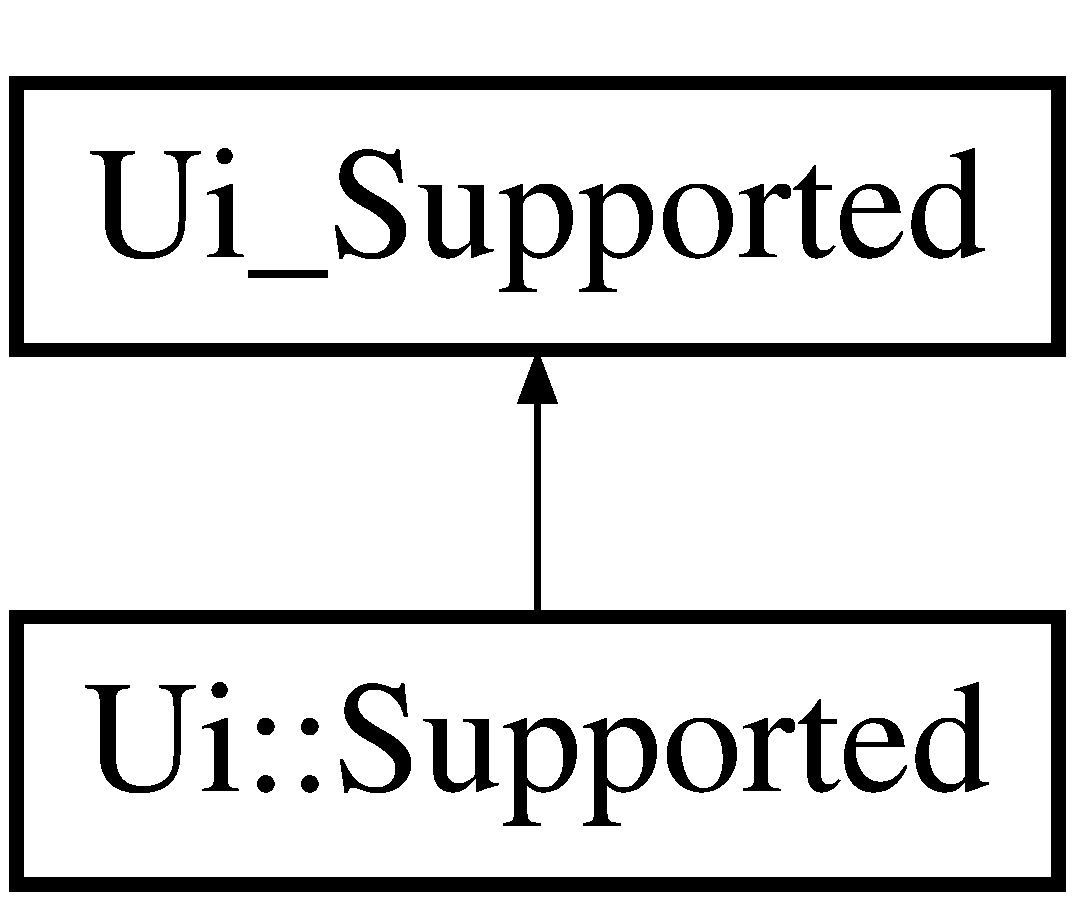
\includegraphics[height=2.000000cm]{classUi__Supported}
\end{center}
\end{figure}
\subsection*{Public Member Functions}
\begin{DoxyCompactItemize}
\item 
\hypertarget{classUi__Supported_a97569a1f269f7af6bd8c4a7664c79d43}{void {\bfseries setup\-Ui} (Q\-Dialog $\ast$\hyperlink{classSupported}{Supported})}\label{classUi__Supported_a97569a1f269f7af6bd8c4a7664c79d43}

\item 
\hypertarget{classUi__Supported_a5875ee5d52f72627137f1e489a5890a8}{void {\bfseries retranslate\-Ui} (Q\-Dialog $\ast$\hyperlink{classSupported}{Supported})}\label{classUi__Supported_a5875ee5d52f72627137f1e489a5890a8}

\end{DoxyCompactItemize}
\subsection*{Public Attributes}
\begin{DoxyCompactItemize}
\item 
\hypertarget{classUi__Supported_ac7aa189fec1d67ba3fbea31b730abb72}{Q\-Table\-View $\ast$ {\bfseries table\-View}}\label{classUi__Supported_ac7aa189fec1d67ba3fbea31b730abb72}

\item 
\hypertarget{classUi__Supported_a270091ee90ddf75c6ef5ad76fcc411c0}{Q\-Combo\-Box $\ast$ {\bfseries cb\-\_\-sel\-\_\-hardware}}\label{classUi__Supported_a270091ee90ddf75c6ef5ad76fcc411c0}

\item 
\hypertarget{classUi__Supported_a2f0ab8f35cdd5ae9ef54517adcb60b26}{Q\-Label $\ast$ {\bfseries l\-\_\-vendor}}\label{classUi__Supported_a2f0ab8f35cdd5ae9ef54517adcb60b26}

\item 
\hypertarget{classUi__Supported_aaad0450a19103f71bc5943f2de044fff}{Q\-Label $\ast$ {\bfseries l\-\_\-custom}}\label{classUi__Supported_aaad0450a19103f71bc5943f2de044fff}

\item 
\hypertarget{classUi__Supported_a841c995091775251005023bc1ebea98e}{Q\-Label $\ast$ {\bfseries l\-\_\-name}}\label{classUi__Supported_a841c995091775251005023bc1ebea98e}

\item 
\hypertarget{classUi__Supported_ac7bfdefacad306bc1cb550c799ccee1f}{Q\-Combo\-Box $\ast$ {\bfseries cb\-\_\-sel\-\_\-vendor}}\label{classUi__Supported_ac7bfdefacad306bc1cb550c799ccee1f}

\item 
\hypertarget{classUi__Supported_ab3fcf2b6fdf3e03ac0283581ef9e039d}{Q\-Combo\-Box $\ast$ {\bfseries cb\-\_\-sel\-\_\-custom}}\label{classUi__Supported_ab3fcf2b6fdf3e03ac0283581ef9e039d}

\item 
\hypertarget{classUi__Supported_ac5bfa65141b0e179f95506575b96f3ed}{Q\-Line\-Edit $\ast$ {\bfseries edit\-\_\-name}}\label{classUi__Supported_ac5bfa65141b0e179f95506575b96f3ed}

\item 
\hypertarget{classUi__Supported_a79c8fffd8ccef6f39108ef7a7a9d0328}{Q\-Label $\ast$ {\bfseries label}}\label{classUi__Supported_a79c8fffd8ccef6f39108ef7a7a9d0328}

\end{DoxyCompactItemize}


The documentation for this class was generated from the following file\-:\begin{DoxyCompactItemize}
\item 
ui\-\_\-supported.\-h\end{DoxyCompactItemize}

%--- End generated contents ---

% Index
\newpage
\phantomsection
\addcontentsline{toc}{chapter}{Index}
\printindex

\end{document}
